%*******************************************************************************
%****************************** Fifth Chapter *********************************
%*******************************************************************************

\chapter{Cosmic Muon Tomography}\label{chp:cosmicMuTelescopes}

\ifpdf
    \graphicspath{{Chapter5/Figs/Raster/}{Chapter5/Figs/PDF/}{Chapter5/Figs/}}
\else
    \graphicspath{{Chapter5/Figs/Vector/}{Chapter5/Figs/}}
\fi

% In spherical polar coordinates, there is also a polar angle commonly denoted as $\theta$. Figure \ref{fig:sphericalPolarCoordinateSystem} shows the coordinate system in $\phi$ and $\theta$ being used

% This chapter is an overview of cosmic muon tomography and an overview of the MU-RAY and DIAPHANE detectors. It will cover the techniques that both collaborations use and why the ``transmission'' technique from the MU-RAY collaboration is especially valuable.

Due to COVID-19 pandemic the focus of the Ph.D. had to change, the upgrade stalled as global supply chains failed. But this afforded an opportunity to revisit the  data set taken at the Wylfa reactor site and attempt cosmic muon tomography. But first the topic of cosmic muon tomography needs to be well understood and in this chapter an overview of cosmic muon tomography follows. This includes the production of cosmic muons in the atmosphere and various fields that use tomography. In general, there are two distinct forms of cosmic muon tomography, two-sided and one-sided and their advantages and disadvantages will will be discussed here. In addition, three main applications of cosmic muon tomography will be considered in this chapter, two-sided reactor tomography, one-sided reactor tomography, and one-sided geological tomography. Cosmic muon tomography allows for positional reconstruction of a detectors surroundings. This positional reconstruction is useful because it guards against a detector from being clandestinely relocated. 

%Whilst during specific short term events the number of solar cosmic rays penetrating the atmosphere can be several orders of magnitude higher than the flux of Galactic cosmic rays the energy of solar events is much lower than the Galactic events \cite{muscheler2013_10be}.

\section{Production Of Cosmic Muons In The Atmosphere} 
Atmospheric muons are produced when high energy protons interact with nuclei in the atmosphere\cite{griffiths2008neutrinoOscillations}. Spallation of atmospheric atom produce cosmic showers an example of which  can be seen in figure \ref{fig:muonShower}. This shows how the production of positive and negative pions from the initial proton interaction leads to the production of positive and negative muon particles (equation \ref{equ:pi+-atmos}) \cite{griffiths2008neutrinoOscillations}. Extra-galactic particles are rare and typically have high energies of $\sim$ $3 \times 10^{18}$ GeV \cite{Drury2012OCosmicRays} \cite{ieee_cry_2007}. Solar particles can be largely disregarded as they are only a significant part of the distribution during solar flares, which are rare \cite{Zyla_pdg_2020} \cite{ieee_cry_2007}. In general, cosmic rays observed at  relativistic energies $> 1\,\textrm{GeV}$ are of exclusively Galactic \footnote{Galaxy with a capital G is used to denote it is the Milky-Way Galaxy that is being discussed.} origin \cite{Drury2012OCosmicRays}. Supernovae are considered to be the main source of Galactic cosmic rays as they are the most viable candidates to produce particles with such energy\cite{Drury2012OCosmicRays}. The distribution of Galactic cosmic rays interacting with the Earth's atmosphere is near isotropic, modulated slowly by variations in the magnetic field produced by the solar wind \cite{Zyla_pdg_2020}. Typically, the kinetic energy for positive and negative muons produced by these Galactic cosmic rays is $\sim$ 4\,GeV in the atmosphere \cite{Zyla_pdg_2020} \cite{MuonPhysics}. The CRY library simulation is derived from full MCNPX simulations and is benchmarked against measured data and gives the energy distribution of muons at sea level shown in fig \ref{fig:keMevCryMuons}. The distribution extends from $\sim$ 100\,MeV to $\sim$ 40 GeV peaking at $\sim$ 1 GeV, which matches the measured distribution \cite{ieee_cry_2007} \cite{Zyla_pdg_2020}. The author’s 6 month placement at A.W.E (see appendix \ref{appen:AweReportOnCosmicMu}) used the CRY library to predict interaction in an idealised detector.\footnote{Appendix \ref{appen:AweReportOnCosmicMu} is a casual internal report designed to explain the work to a hand-off scientist it is not written to the same standard as this thesis.}.

% Atmospheric muon are produced when high energy protons interact with nuclei in the atmosphere \cite{griffiths2008neutrinoOscillations}. An example of a cosmic shower can be seen in figure \ref{fig:muonShower}, which shows how the production of positive and negative pions from the initial proton interaction leads to the production of $\mu^-$ and $\mu^+$ particles (equation \ref{equ:pi+-atmos}) \cite{griffiths2008neutrinoOscillations}. There are three main sources of cosmic protons: solar, Galactic, and extra-Galactic \cite{Drury2012OCosmicRays} \cite{muscheler2013_10be} \cite{Pierre2017Aniostropy}. Extra-Galactic particles are rare and typically have high energies of $\sim$ 10$^{18}$\,eV \cite{Pierre2017Aniostropy}. In general, cosmic rays observed at mildly relativistic energies, around 1\,GeV per nucleon are of exclusively Galactic origin \cite{Drury2012OCosmicRays}. Supernovae are considered to be the main source of Galactic cosmic rays as they are the most viable candidates to produce particles with such energy \cite{Drury2012OCosmicRays}. Typically the kinetic energy for $\mu^-$ and $\mu^+$ is $\sim$ 4\,GeV in the atmosphere \cite{MuonPhysics} \cite{ieee_cry_2007}. Therefore, for most cosmic rays it is reasonable to assume Galactic origin, and as such the onset of night at any given site may have little effect on cosmic muon production. This assumption is also reinforced by the CRY library where $\sim 80\,\%$ are above 1\,GeV. Though it is possible for a solar proton event to produce a flux of muon that exceeds the galactic flux of protons (at least at the poles) they are typically of much lower energies \cite{muscheler2013_10be}. Sources focusing on solar proton events tend to focus on particles with energy $\geq$ 30\,MeV \cite{Panasyuk_NERSolar_2018} \cite{gabriel1990periodicities}. So between 30\,MeV and 1\,GeV solar activity could have an impact on proton production and thus atmospheric muon production depending on how active the sun is at any given time. Typically cosmic muon are treated as noise and are often characterised to gain an understanding of their contribution to the background. For example, his was done during the author's 6 month placement at A.W.E (see appendix \ref{appen:AweReportOnCosmicMu})\footnote{Appendix \ref{appen:AweReportOnCosmicMu} is a casual internal report designed to explain the work to a hand-off scientist it is not written to the same standard as this thesis.}.

\begin{figure}[!h]
 \centering
 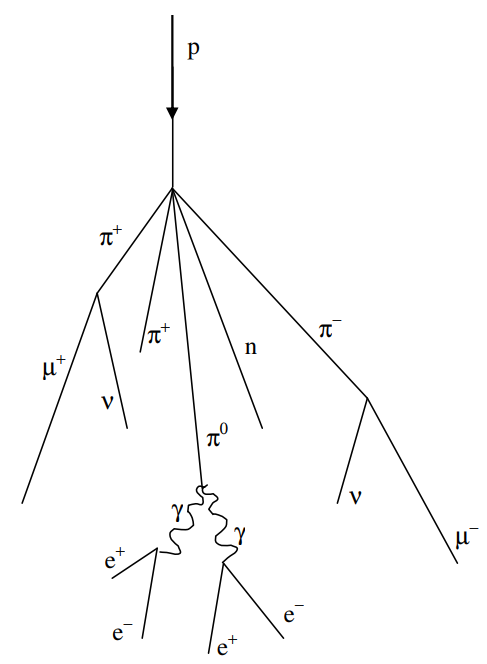
\includegraphics[width=0.3333\linewidth]{Chapter5/Figs/Raster/muonShower.png}
 \captionof{figure}[An illustration of the shower of particles produced by cosmic ray collisions.]{An illustration of the shower of particles produced by cosmic ray collisions. Atmospheric muons are produced from the secondary positive and negative pions in the atmosphere which are in turn produced from hadronic collisions with protons and atmospheric nuclei. From \cite{MuonPhysics}.}
 \label{fig:muonShower}
\end{figure}

\begin{equation}
  \pi^+ \rightarrow \mu^+ + \nu_\mu  \qquad \qquad \pi^- \rightarrow \mu^- + \Bar{\nu_\mu} 
  \label{equ:pi+-atmos}
\end{equation}

\section{Overview Of Cosmic Muon Tomography}\label{sec:cosMuOverview}
%What is cosmic muon tomography? What does the process include? 
%Whats the difference between muon tomography and muon radiography?

%The principle novelty of cosmic muon tomography is the ability to measure the angles of arriving cosmic ray muon with great precision over a sensitive area \cite{Alvarez_Pyramids_1970}. One of the first and most notable uses for cosmic muon tomography was imaging the second pyramid of Giza in 1970 \cite{Alvarez_Pyramids_1970}. One of the major concerns surrounding cosmic muon tomography was and still is the amount of scattering caused from measuring high z materials \cite{Alvarez_Pyramids_1970}. Cosmic muon tomography requires the use of precise instrumentation to accurately resolve the incoming particles. For example, the advent of spark chambers was required for pyramid imaging \cite{Alvarez_Pyramids_1970}. 

Cosmic muon tomography uses measurements of the cosmic muon flux to image massive objects in the path of cosmic rays to the detectors. The changes in expected muon flux due to absorption and scattering of cosmic rays in material before the detector are related to the quantity and density of material present. Cosmic muon tomography relies on  the ability to measure the angles of the arriving cosmic muons with great precision over a sensitive area \cite{Alvarez_Pyramids_1970}. One of the first and most notable uses for cosmic muon tomography was imaging the second pyramid of Giza in 1970 \cite{Alvarez_Pyramids_1970}. To achieve angular resolution sufficient for pyramid imaging, spark chambers were used \cite{Alvarez_Pyramids_1970}. Whilst the results from the pyramid were disappointing as they proved that there was no hidden chamber it was still useful as it did so without excavation and damage to a world famous land mark \cite{Alvarez_Pyramids_1970}. 
%Cosmic muon tomography allows for positional reconstruction of a detectors surroundings. This positional reconstruction is useful because it guards against the detector from being forcibly relocated. %bag for later
\\\\Electron anti-neutrinos cannot be obscured due to their small cross-section of 10$^{-42}$\,cm$^2$ \cite{Vogel_1999}. As a result the only method to deceive an electron anti-neutrino detector (bar tampering) is to relocate it. GPS trackers are a solution but can be potentially jammed therefore positional guarding via cosmic muon tomography is desirable. A time of 1\,hour per week was targeted to obtain enough events to not be limited by statistical uncertainty whilst being unobtrusive to electron anti-neutrino reactor monitoring. Typically the refuelling of a reactor takes about 1 month for PWRs and BWRs therefore 1 hour a week is more than sufficient \cite{CHANG_1999_simpRefuel}. For other online refuelling reactor types the situation is more complex. Instead, it may be more prudent to increase the muon tomography rate to 15 minutes per 24 hours of reactor time. As the reactor will have to wait 40-50 hours for the xenon in the core to stabilise once fuel has been removed \cite{doeHandbook1993NucReac}. Fortunately, cosmic muon events were taken in accidental coincidence during the Wylfa deployment; this afforded a fantastic opportunity to test the tomographic capabilities of the detector. To that end an overview of other detectors will follow to assess the limitations of this approach. 
\\\\Cosmic muon tomography can be split into two distinct types, one-sided and two-sided. Two-sided cosmic muon tomography measures the incoming muon angles and outgoing muon angles over a given area with an object of interest to be imaged as shown by figure \ref{fig:twoSidedCosmicMuonTomographySchults}. This approach allows for vertex reconstruction and measures cosmic muon scattering thus giving a detailed interior image of the object being imaged \cite{schultz_2007}. Two-sided cosmic muon tomography has been used to analyse nuclear waste \cite{jonkmans2013nuclear} and even imaging the Fukushima Daiichi reactors \cite{miyadera2013imaging}. However, as figure \ref{fig:twoSidedCosmicMuonTomographySchults} shows the  detectors are typically much larger or of similar size to the object that they are attempting to image. So whilst this technique would yield a very accurate breakdown of the internal structure of any given object it would not be suitable in all cases. For example, if an object of interest is much larger than the detector only a small portion of it can be analysed. 

\begin{figure}[!h]
 \centering
 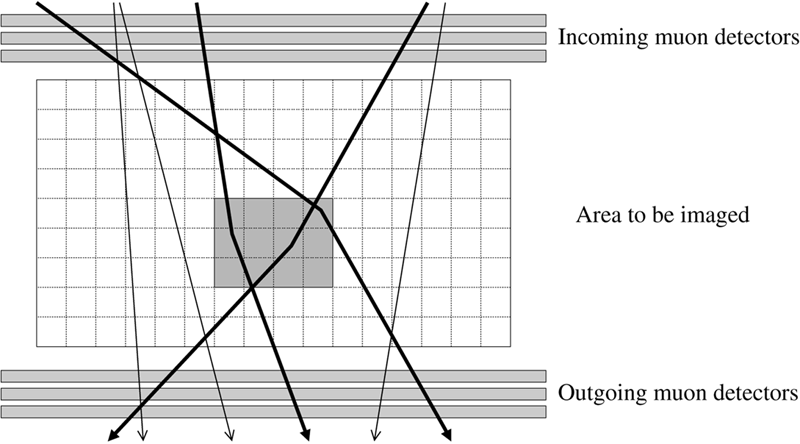
\includegraphics[width=0.7\linewidth]{Chapter5/Figs/Raster/twoSidedCosmicMuon_schults2007.png}
 \captionof{figure}[A side-on view of two-sided cosmic muon tomography.]{A side-on view of two-sided cosmic muon tomography, the detectors are of similar size or larger than the object that is being measured in order to make coincided measurements using cosmic muons seen in the scattered (black) cosmic muons. From \cite{schultz_2007}.}
 \label{fig:twoSidedCosmicMuonTomographySchults}
\end{figure}
 
%  \begin{figure}[!h]
%  \centering
%  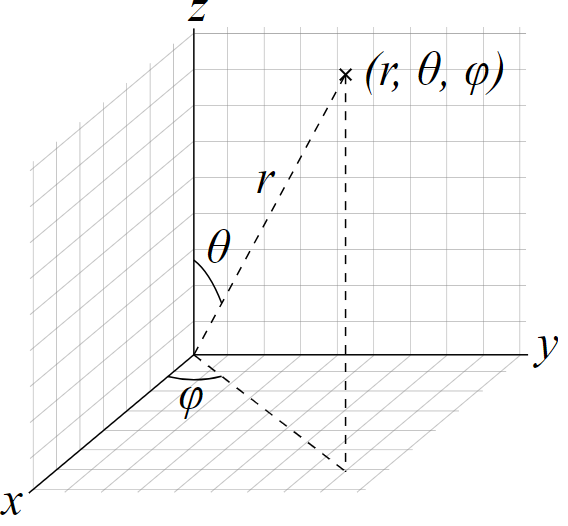
\includegraphics[width=0.3\linewidth]{Chapter5/Figs/wylfaRasterNew/sphericalPolarCoordinatesystem.png}
%  \captionof{figure}{The spherical polar coordinate system is typically used in physics with the azimuthal angle denoted by $\phi$ and the polar angle denoted by $\theta$. Taken from Wikipedia \cite{wikipeidaSphericalCoordinateSystem}.} 
%  \label{fig:sphericalPolarCoordinateSystem}
% \end{figure}
 
 One-sided cosmic muon tomography is where one detector is used to measure the cosmic muon incidence, a simplistic example can be seen in figure \ref{subFig:TopDownCircularWallPlot}. Figure \ref{subFig:TopDownCircularWallPlot} is an extremely simplified case where there is a singular wall that blocks 50\,\% of cosmic muon incidence. However, such a scenario is unlikely except for extremely high Z materials \cite{schultz_2007}. A more realistic example would be in figure \ref{subFig:TopDownCircularCubePlot} where the decreasing attenuation corresponds to more material producing a curve shape in the occluded angles of $\phi$. The top-down perspective in figures \ref{subFig:TopDownCircularWallPlot} and \ref{subFig:TopDownCircularCubePlot} only show the azimuthal angle ($\phi$). 
 
 \begin{figure}[!h]
\centering
\begin{subfigure}{.5\textwidth}
  \centering
  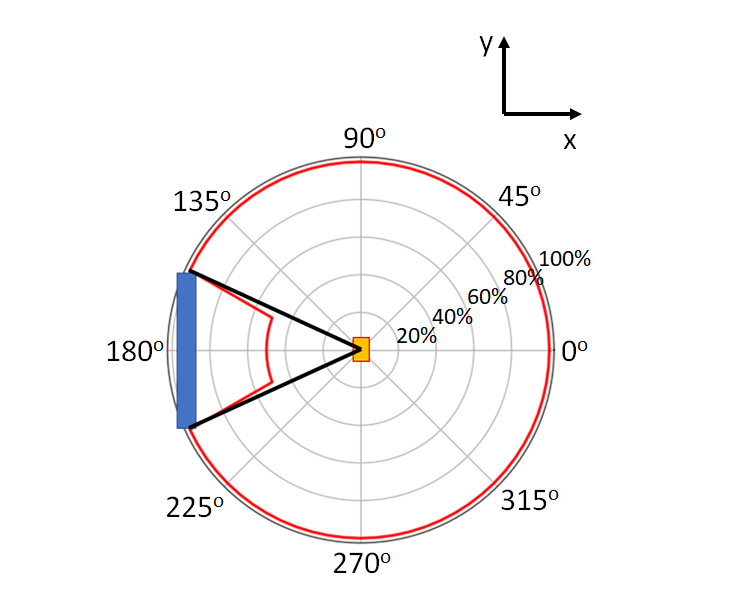
\includegraphics[width=\linewidth]{Chapter5/Figs/topDownWallPhiRedo.png}
  \captionsetup{width=.9\linewidth}
  \caption{}
  \label{subFig:TopDownCircularWallPlot}
\end{subfigure}%
\begin{subfigure}{.5\textwidth}
  \centering
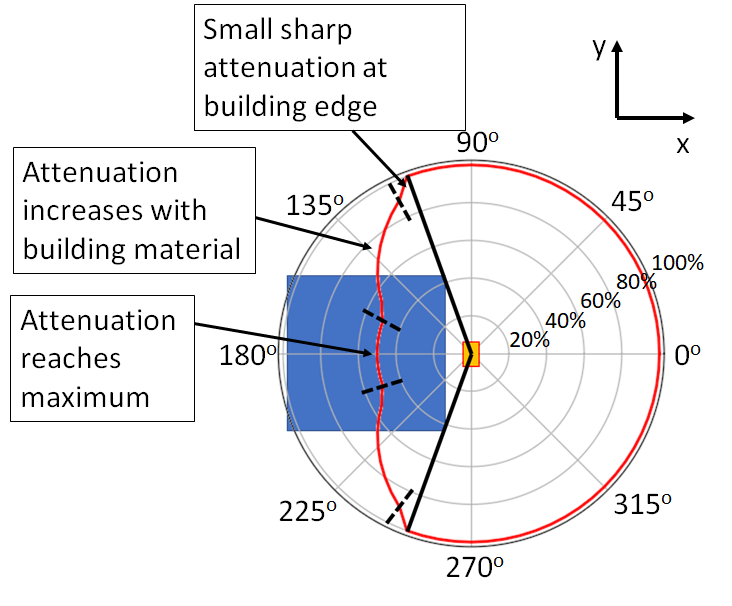
\includegraphics[width=\linewidth]{Chapter5/Figs/topDownCubePhiRedo.png}
  \captionsetup{width=.9\linewidth}
  \caption{}
  \label{subFig:TopDownCircularCubePlot}
\end{subfigure}
\caption[Top down examples of one-sided cosmic muon tomography.]{Top down examples of one-sided cosmic muon tomography. (a) shows how a thin dense wall that blocks 50\,\% of cosmic muon incidence would look, a sharp drop in incidence at the edges with no further attenuation. (b) How a cube of material would block cosmic muon incidence would look, the amount of attenuation corresponds to the amount of material in the path of the cosmic muon.}
\label{fig:TopDownCircularWallCubePlot}
\end{figure}
 
 \begin{figure}[!h]
 \centering
 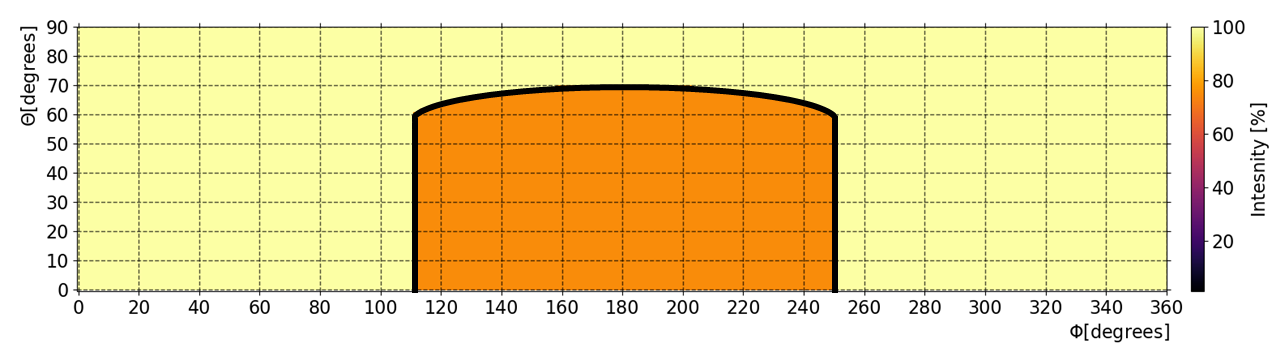
\includegraphics[width=\linewidth]{Chapter5/Figs/wylfaRasterNew/phiVsThetaExpectedInferno_outlined.png}
 \captionof{figure}[Top down example of one-sided cosmic muon tomography, represented in $\theta$ and $\phi$.]{How the example seen in figure \ref{subFig:TopDownCircularCubePlot} can be represented in $\theta$ and $\phi$, assuming it's a cuboid.} 
 \label{fig:thetaVsPhiExpectedCube}
\end{figure}

When imaging a cuboid, straight line edges in $\phi$ may be seen, from the sides of the cuboid. The top edge of the cuboid is imaged as a curve, showing that as the distance from the origin changes along the edge, the height is constant so the angle polar angle ($\theta$) varies. If figure \ref{subFig:TopDownCircularCubePlot} is taken and analysed in both $\phi$ and $\theta$ a 360$^\circ$ panoramic view is produced (figure \ref{fig:thetaVsPhiExpectedCube}). In the idealised example, shown in figure \ref{fig:thetaVsPhiExpectedCube}, the attenuation is held constant. In a more realistic model, the attenuation will be dependent on the distance travelled by muon in the cuboid leading to angular dependence on the attenuation seen. Close to the edges of the cuboid, the attenuation will be seen to smoothly drop to zero due to geometric effects. This example is designed to show that even under ideal circumstances there is inherent distortion when analysing the whole cosmic muon hemisphere at once. This distortion is due to the detector in this example acting more as a 360$^\circ$ cosmic muon camera rather than a cosmic muon telescope in the strictest sense.
\\\\Further, it is important to recognise that the muon scattering angle ($\theta_s$) is different for different atoms \cite{Liu2020MuonScatteringZ} \cite{tripathy2016understanding}. The angular scattering distribution is given by equation \ref{equ:fTheta}. This distribution is a Gaussian where elements with a larger atomic number (Z) will have a broader peak and elements with a smaller atomic number will have a more defined peak \cite{Liu2020MuonScatteringZ}. This distribution represents multi-Coulomb scattering \cite{Liu2020MuonScatteringZ}, \cite{tripathy2016understanding} where the root mean square error $\sigma_\theta_s$ is given by equation \ref{equ:sigmaTheta}. Finally the radiation length (the mean length (in cm) of a material to reduce the energy of an electron by a factor 1/$e$ denoted by L$_{\textrm{rad}}$) is given by equation \ref{equ:lRad}. Equation \ref{equ:lRad} is a widely used empirical equation \cite{Liu2020MuonScatteringZ} \cite{tripathy2016understanding}. It should be noted that this is how GEANT4 models muons scattering \cite{tripathy2016understanding}.
\begin{equation}
    f(\theta_s) = \frac{1}{\sqrt{2\pi}\sigma_\theta_s} \exp\left({-\frac{\theta_s^2}{2\sigma_{\theta_s}^2}}\right)
    \label{equ:fTheta}
\end{equation}
\begin{equation}
    \sigma_\theta_s = \frac{13.6\,\textrm{MeV}}{\beta c p} \sqrt{\frac{L}{L_\textrm{rad}}}\left[1 + 0.038\ln{\left(\frac{L}{L_\textrm{rad}}\right)}\right]  
    \label{equ:sigmaTheta}
\end{equation}
\begin{equation}
    L_\textrm{rad} = \frac{716.4\,\cdot\, A}{Z(Z+1)\ln{(287/\sqrt{Z})}} [\textrm{g}/\textrm{cm}^3]
    \label{equ:lRad}
\end{equation}
%For figure \ref{fig:thetaVsPhiExpectedCube} there is a slight distortion caused at the top of the building due to the projection of a hemispherical distribution onto a cuboid detector. The amount of distortion will also vary depending on the distance from the detector and the size and shape of the building in question. Longer shorter buildings will have significantly mor top distortion than tall narrow buildings. The slope of the distortion will also vary depending on the position relative to the detector. Further, in figure \ref{fig:thetaVsPhiExpectedCube} the drop in intensity would not be expected to be instantaneous, there would be a gradual decrease in intensity resulting in blurred edges around the occlusion pattern or ``shadow.'' These effects will vary depending on the setup. The VIDARR and RMon detectors for example are cuboid detectors that analyse the whole hemisphere at once, and as such can be considered as 360$^\circ$ cosmic camera rather than as a cosmic muon telescope in the strictest sense. This is an important consideration as the other cosmic muon experiments have very different experimental setups. As will be seen in section \ref{sec:muTomographyExamples}.

\section{Muon Tomography Examples} \label{sec:muTomographyExamples}
There are several fields that utilise cosmic muon tomography. These include archaeology, geological physics, reactor imaging, and nuclear waste imaging. Archaeology requires a large man made structure with potentially hidden rooms, and so is a niche application \cite{Alvarez_Pyramids_1970}. Nuclear waste imaging utilises two-sided cosmic muon tomography to ascertain detailed information \cite{jonkmans2013nuclear}. Two-sided muon tomography is also used for reactor monitoring as the extra information afforded by two-sided tomography is highly desirable \cite{miyadera2013imaging} \cite{perry_imaging_2013} \cite{morris2014analysis}. Though the simplicity and ease of deployment for one-sided tomography does have a case to be made \cite{Erlandson_reactorOST_2018} \cite{Fujii_ReactorRadiography_2019}. As a result, one-sided cosmic muon tomography tends to be most utilised with geological physics and is often extended via muon radiography \cite{Tanaka_mtAsama_2007} \cite{Marteau_2017}. As the detector at Wylfa is significantly smaller than the reactor buildings and only one was deployed, one-sided cosmic muon tomography was used at Wylfa. But for completeness, the use of both two-sided and one-sided reactor tomography are reviewed here to give a full picture of the field. Geological tomography is also covered as the field uses one-sided tomography to build complex density and deficit maps and so is also of interest. 

\subsection{Two-Sided Reactor Muon Tomography}
% Several papers focus on Fukushima \cite{miyadera2013imaging} \cite{morris2014analysis}
% \\useful considering the nature of the incident 
% \\show figure of their proposed deployment fig \ref{fig:fukushimaImaging}
% \\show the mock up of their mini scale reactor fig \ref{fig:fukushimaFakeCore}
% \\also mention the Toshiba critically assemble as it was inspired by this \cite{morris2014analysis} fig \ref{fig:Toshiba3dTomogarphy} fig \ref{fig:toshibaG4Compare}.
% \\the Peri paper also has a feasibility study for this \cite{perry_imaging_2013} (no standout figs)
% %\\finally close off with fig \ref{fig:2dZedCore} showing the ZED-2 core in 2d \cite{Erlandson_reactorOST_2018}
Two-sided reactor tomography came to the forefront after the Fukushima Daiichi disaster in 2011. A need to assess the status of the reactor cores in a non-invasive manner was highly desirable due to the high levels of radiation on site \cite{miyadera2013imaging}. The proposed detectors can be seen in figure \ref{fig:fukushimaImaging} where two detector panels of differing sizes are used for position and density reconstruction \cite{miyadera2013imaging}. In the summer of 2011 a reactor mock-up was imaged using the Muon Mini Tracker (MMT). The MMT consists of two muon trackers each having an effective detection area of 1.2 $\times$ 1.2 m$^2$ and consisting of six-x and six-y planes of sealed drift tubes \cite{miyadera2013imaging}.

\begin{figure}[!h]
 \centering
 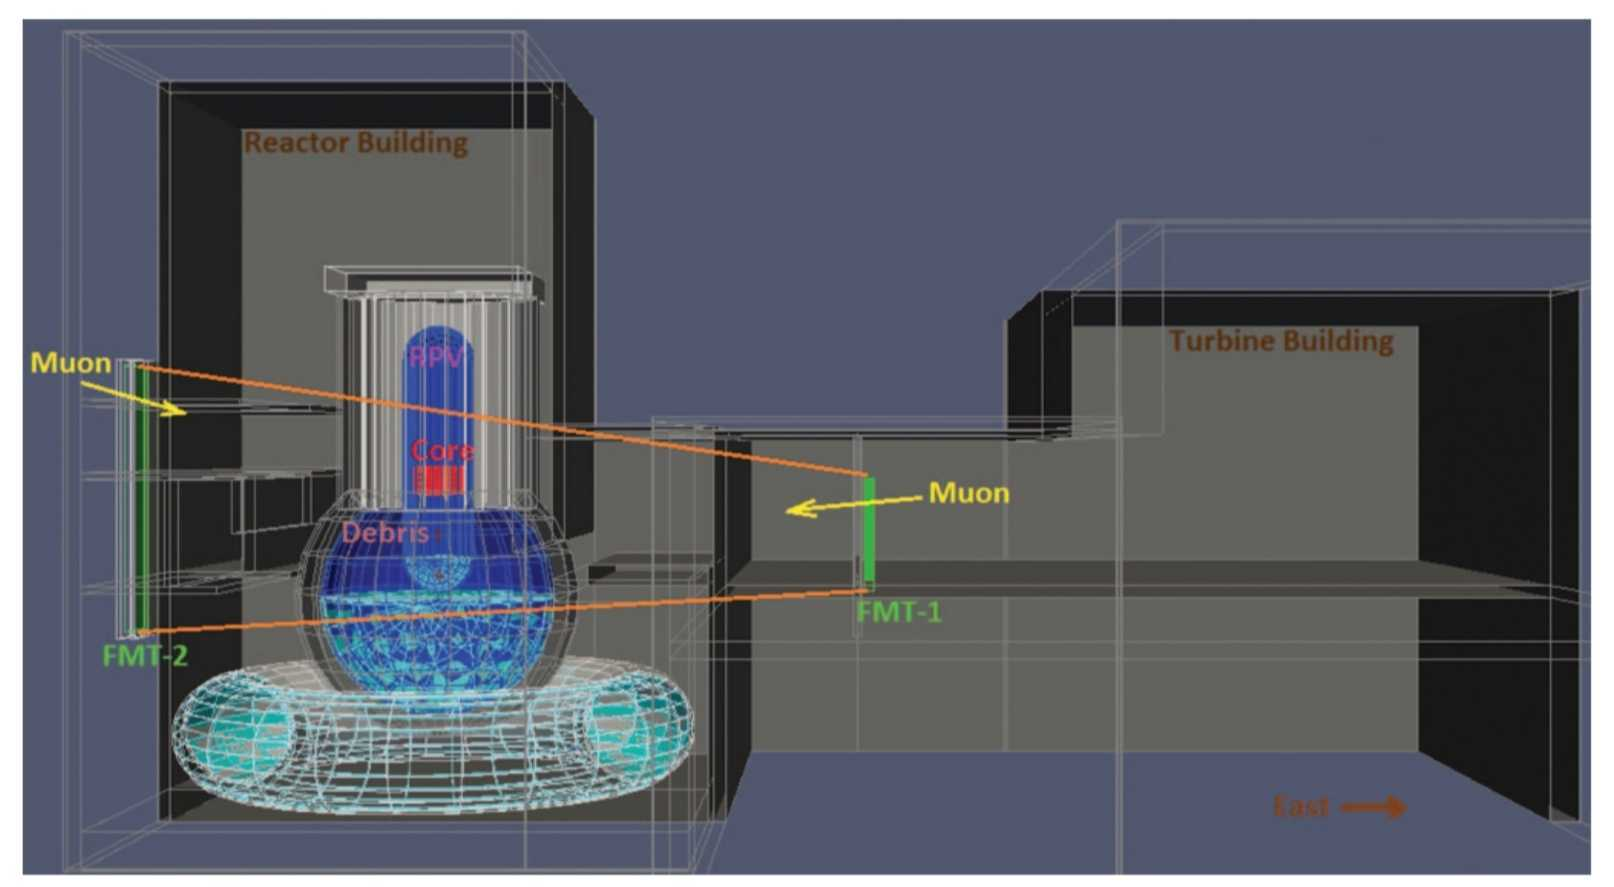
\includegraphics[width=0.7\linewidth]{Chapter5/Figs/MuTomographyExamples/fukushimaImaging.jpg}
 \captionof{figure}[Muon imaging setup for Fukushima Unit 2.]{Muon imaging setup for Fukushima Unit 2. FMT-2 is installed inside a concrete radiation shield in front of the reactor building. muon scatting angles are a few degrees. From \cite{miyadera2013imaging}.} 
 \label{fig:fukushimaImaging}
\end{figure}

A result from the MMT is shown in figure \ref{fig:fukushimaFakeCore} where two-sided muon tomography is able to resolve a conical void similar in shape to the melted core of the Three Mile Island core. This lead core had two layers of concrete shielding blocks with a thickness of 2.74\,m each. Over a 3 week period 8 $\times$ 10$^4$ muon events were accumulated, this is an order of magnitude less than what would be expected from the full deployment at Fukushima. A company was awarded a contract to deploy these detectors at the Fukushima site in August of 2014 \cite{compnayFukushimaWeb}.

\begin{figure}[!h]
 \centering
 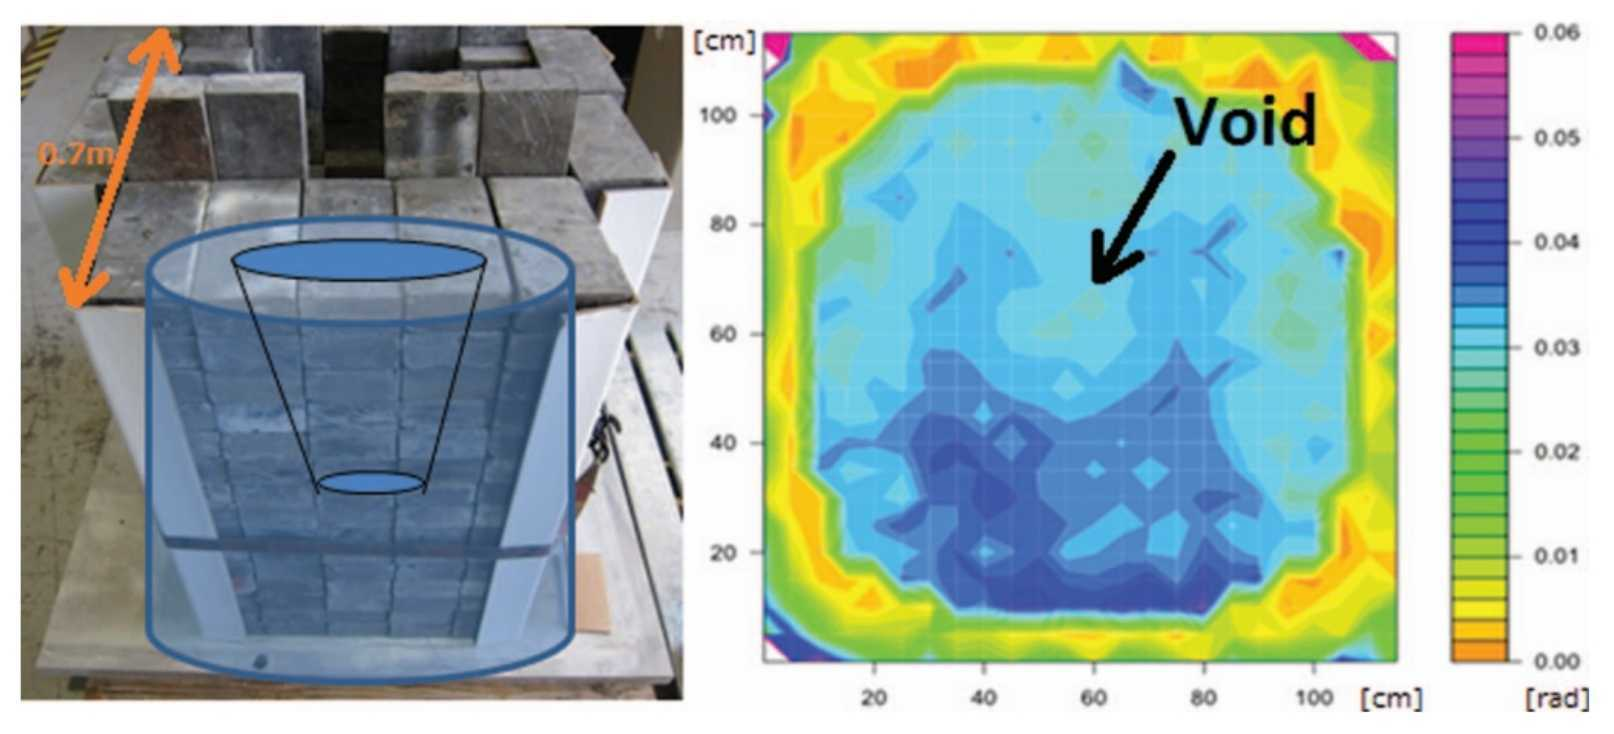
\includegraphics[width=0.7\linewidth]{Chapter5/Figs/MuTomographyExamples/FukushimaFakeCore.jpg}
 \captionof{figure}[Two-sided muon tomography of small example reactor core.]{Two-sided muon tomography of small example reactor core. Left -- Lead reactor core with conic void. Right -- observed core where average scattering angles of muons are plotted. The void in the core is clearly image through 2.74\,m concrete walls. Hot spots at the corners are artefacts caused by edge effects. From \cite{miyadera2013imaging}.} 
 \label{fig:fukushimaFakeCore}
\end{figure}
% Left -- Lead reactor core with conic void. Right -- observed core where average scattering angles of muon are plotted. The void in the core is clearly image through 2.74\,m concrete walls. The lead core of 0.7\,m thickness gives and equivalent radiation length to the uranium fuel in unit 1, and gives a similar scattering angle. Hot spots at the corners are artefacts caused by edge effects. From \cite{miyadera2013imaging}.

The MMT was then moved to the Toshiba facility at Kawasaki, Japan. The MMT was deployed for $\sim$ 4 weeks radiographing the Toshiba Critical Assembly Reactor using cosmic-ray muons \cite{morris2014analysis}. This was done to validate the concept of imaging the damaged cores at Fukushima Daiichi. The configuration for the Toshiba reactor can be seen in figure \ref{fig:Toshiba3dTomogarphy} and is similar to the Fukushima setup. A comparison between GEANT4 Monte Carlo data is also shown in figure \ref{fig:toshibaG4Compare}. The quantitative agreement is within 3\,\% in measured density \cite{morris2014analysis}. These strong agreements show how powerful and robust the results of two-sided cosmic muon tomography are, and why it is desirable if an experiment can deploy multiple detectors and image a significant area. 

\begin{figure}[!h]
\centering
\begin{minipage}{.45\textwidth}
  \centering
  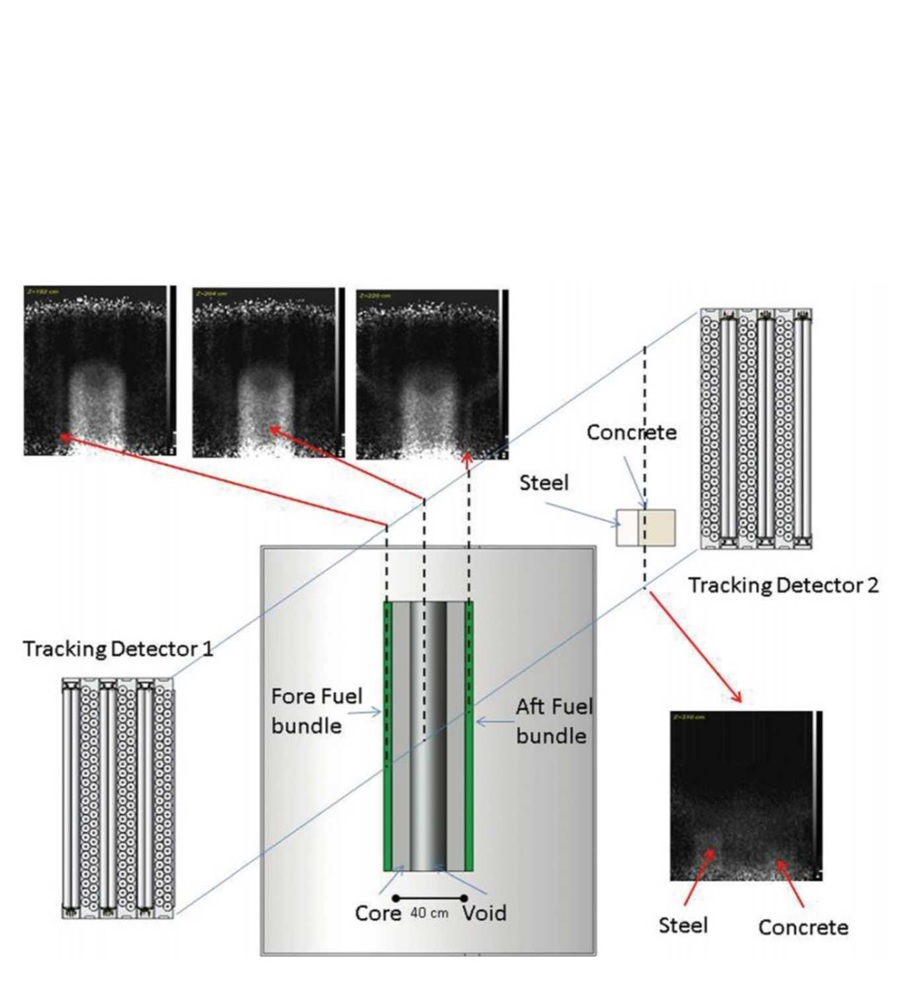
\includegraphics[width=\linewidth]{Chapter5/Figs/MuTomographyExamples/Toshiba3dTomogarphy.jpg}
  \captionof{figure}[Layout and some slices from the three dimension tomograph at TNCA.]{Layout and some slices from the three dimension tomograph showing the major features in the Toshiba Nuclear Critical Assembly reactor image. From \cite{morris2014analysis}.} 
  \label{fig:Toshiba3dTomogarphy}
  \vspace{1.434cm} %1 line = 0.478cm % 2 lines = 0.956cm % 3 lines= 1.434cm % 4 lines = 1.912cm % 5 lines = 2.39cm
\end{minipage}%
\qquad
\begin{minipage}{.45\textwidth}
  \centering
  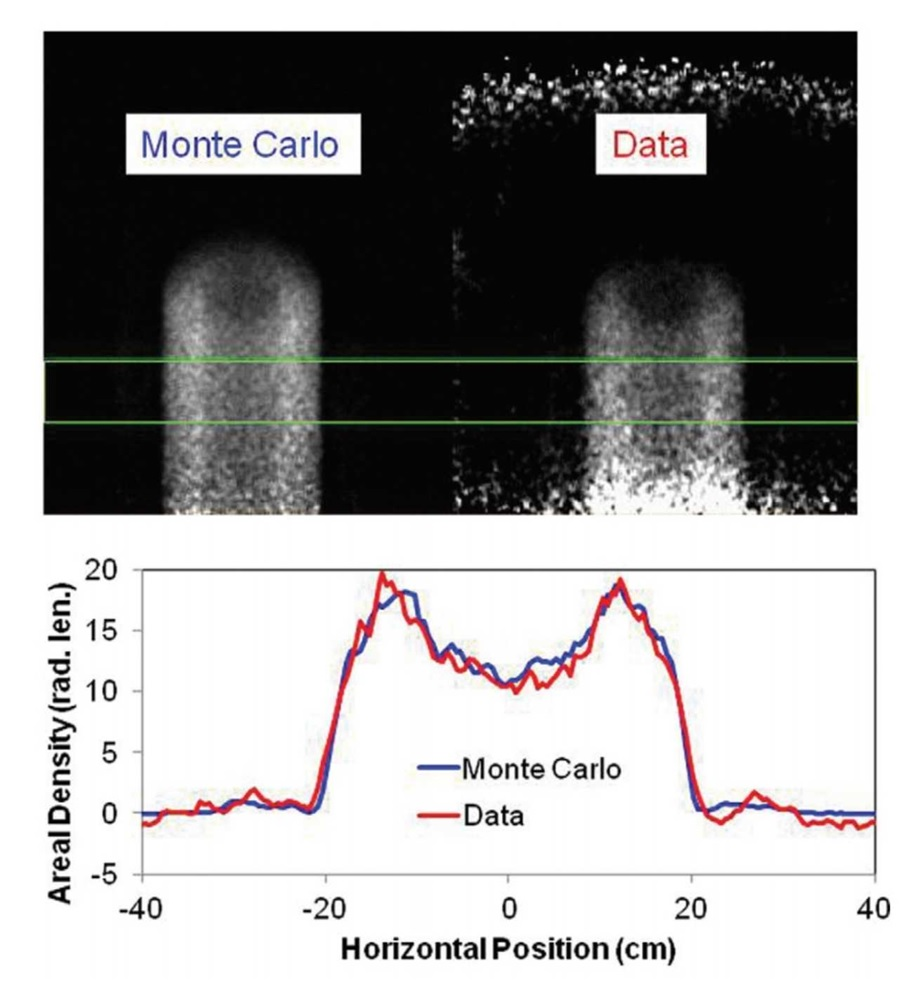
\includegraphics[width=\linewidth]{Chapter5/Figs/MuTomographyExamples/toshibaG4Compare.jpg}
  \captionof{figure}[GEANT4 Monte Carlo simulation vs. data for a slice through the centre of the TNCA reactor core.]{GEANT4 Monte Carlo simulation vs. data for a slice through the centre of the Toshiba Nuclear Critical Assembly reactor core. Top images with the projected region marked by green lines. Bottom plots of the areal density vs. horizontal position. From \cite{morris2014analysis}.}
  \label{fig:toshibaG4Compare}
\end{minipage}
\end{figure}

% \begin{figure}[!h]
%  \centering
%  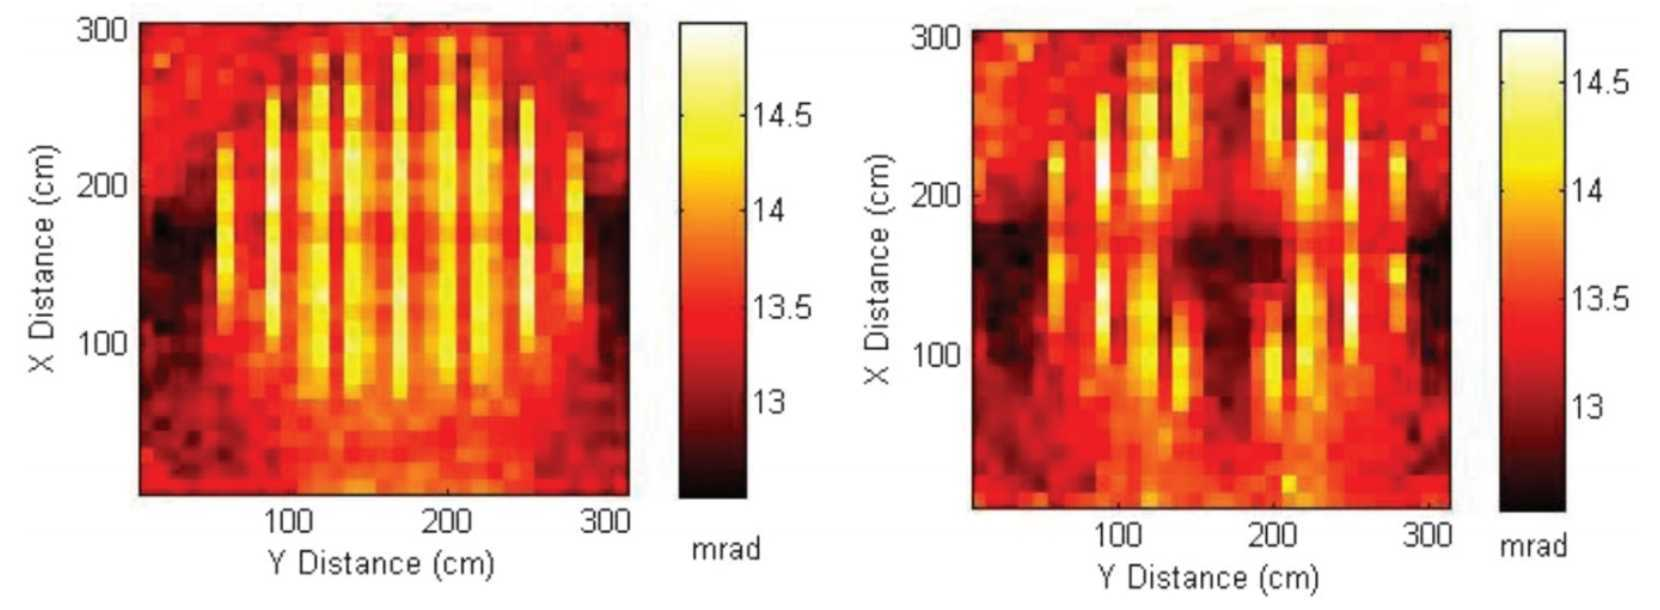
\includegraphics[width=1.0\linewidth]{Chapter5/Figs/MuTomographyExamples/2dZedCore.jpg}
%  \captionof{figure}{Reconstructed images of ZED-2 core during normal operating conditions (left) and a postulated accident scenario (right). Both images were reconstructed using two-sided muon tomography (see figure \ref{fig:Toshiba3dTomogarphy}). From \cite{Erlandson_reactorOST_2018}.} 
%  \label{fig:2dZedCore}
% \end{figure}

%\clearpage
\subsection{One-Sided Reactor Muon Tomography}
% Open up with Canadian paper \cite{Erlandson_reactorOST_2018} 
% \\This reactor has already been imaged via two sided tomography
% \\Talk about benefits of portability and simplicity fig \ref{fig:Zed2Core1dRotation}, \cite{Fujii_ReactorRadiography_2019} 
% \\Then open up with radiography paper \cite{Fujii_ReactorRadiography_2019}
% \\Then mention the imaging of the reactor using one-sided tomography fig \ref{fig:JapcNuclearPowerImaging}, fig \ref{fig:JapcMt2Data} 
Whilst the benefits of two-sided tomography cannot be ignored there are distinct advantages to one-sided tomography. The comparative ease of deployment, ease of moving the detector or detector array, and multiple angles of measurement could allow for better tomography providing the correct approach is taken \cite{Erlandson_reactorOST_2018}. Unlike two-sided reactor tomography one-sided reactor tomography needs to be rotated around a reactor core to give a complete status of the core see figure \ref{fig:Zed2Core1dRotation} \cite{Erlandson_reactorOST_2018}. 

% \begin{figure}[!h]
%  \centering
%  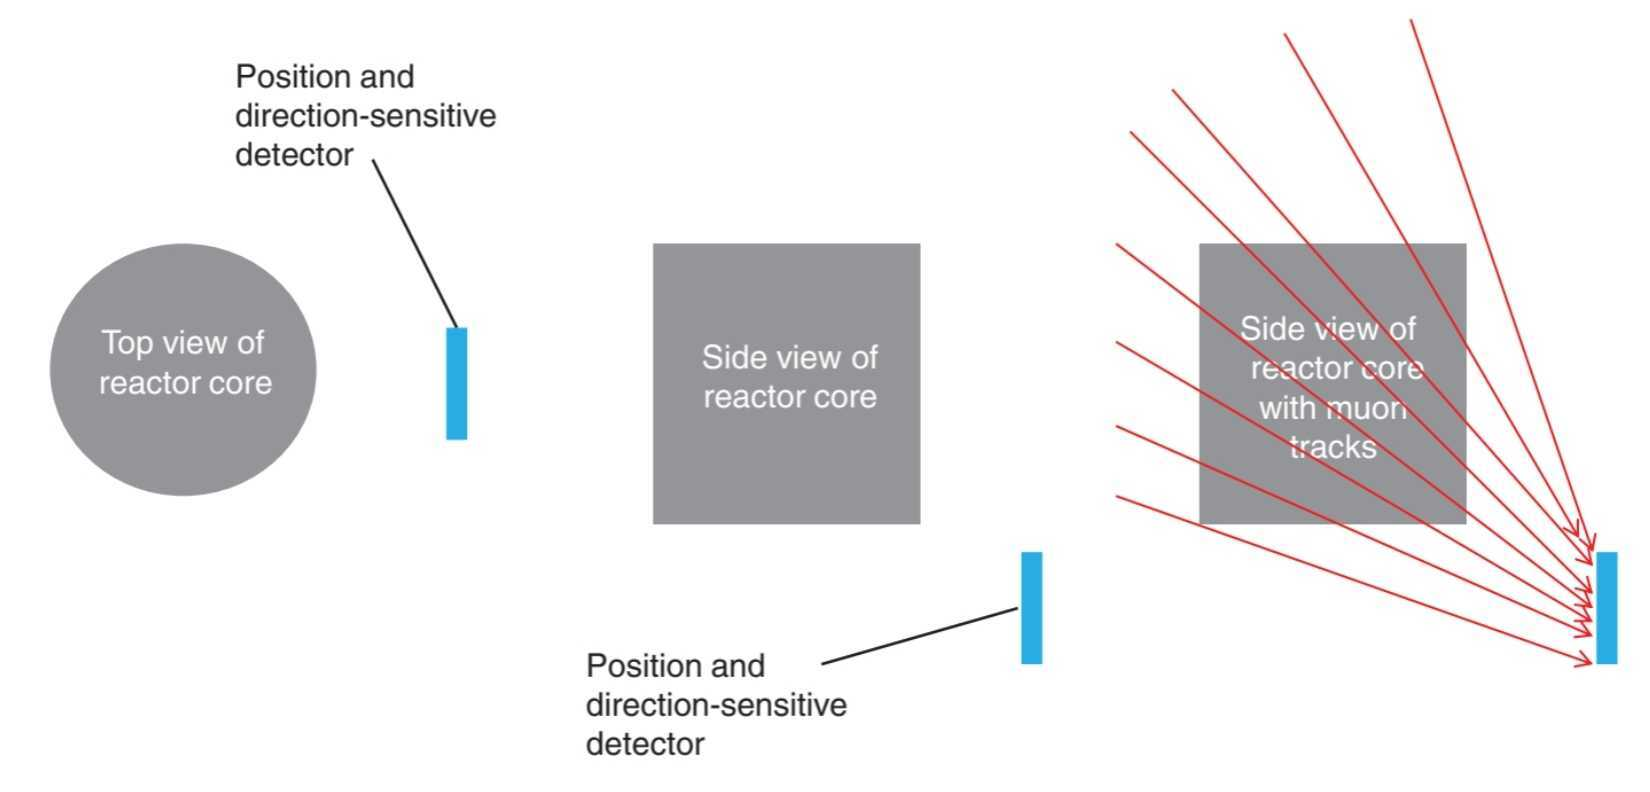
\includegraphics[width=0.8\linewidth]{Chapter5/Figs/MuTomographyExamples/ZdExplainationOf1D.jpg}
%  \captionof{figure}{Geometrical setup for the one-sided muon tomography concept.} 
%  \label{fig:ZdExplainationOf1D}
% \end{figure}

\begin{figure}[!h]
 \centering
 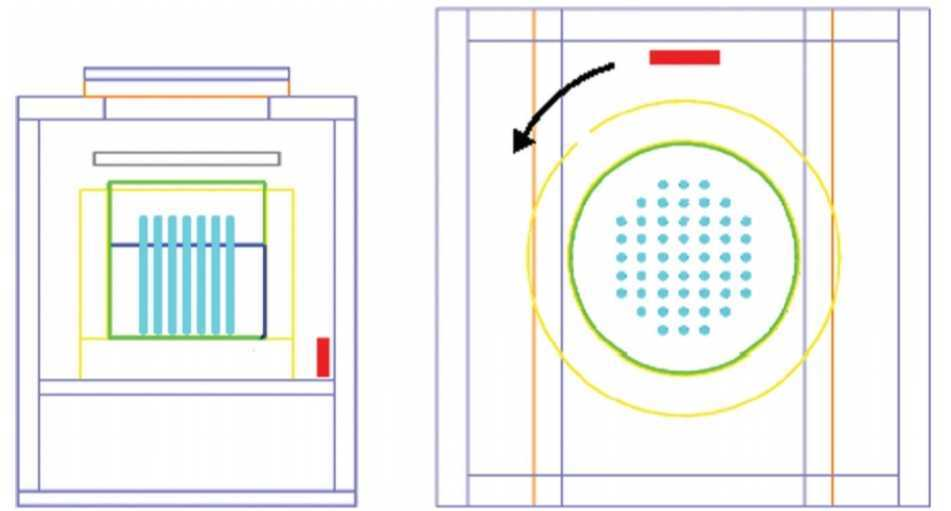
\includegraphics[width=0.7\linewidth]{Chapter5/Figs/MuTomographyExamples/Zed2Core1dRotation.jpg}
 \captionof{figure}[Detector placement for one-sided muon tomography of the ZED-D reactor.]{Detector placement for one-sided muon tomography of the ZED-D reactor. left: side-view. Right: top-view. From \cite{Erlandson_reactorOST_2018}.} 
 \label{fig:Zed2Core1dRotation}
\end{figure}

By simulating the ZED2 Canadian reactor core in GEANT4, Erlandson et al. were able to image the core (see figure \ref{fig:Zed2OstSimulation}) \cite{Erlandson_reactorOST_2018}, investigating changes, such as any damage to the core assembly. The simulated reconstruction was done using the algebraic reconstruction technique (ART). This technique has two key inaccuracies seen in the middle row in figure \ref{fig:Zed2OstSimulation}. The first is the low density that has been reconstructed in the centre of the core. The second is the oscillating pattern of high density material where the fuel is present due to the twelve positions simulated for imaging the core overlapping slightly \cite{Erlandson_reactorOST_2018} . These problems are overcome by taking a control data set before any damage and then subtracting that control distribution (left column of figure \ref{fig:Zed2OstSimulation}) from the ART results (middle row of figure \ref{fig:Zed2OstSimulation}) producing the bottom row of figure \ref{fig:Zed2OstSimulation} which clearly shows the damage in the core \cite{Erlandson_reactorOST_2018}. This technique requires more time ($\sim$ 33 days) than two-sided tomography ($\sim$ 5 days). But the size and cost of the proposed one-sided detectors is significantly lower then that of the equivalent two-sided method \cite{Erlandson_reactorOST_2018}. 
%This technique is of particular interest as rotating as rotating around a building to image it is very possible for VIDARR in a future deployment.

\begin{figure}[!h]
 \centering
 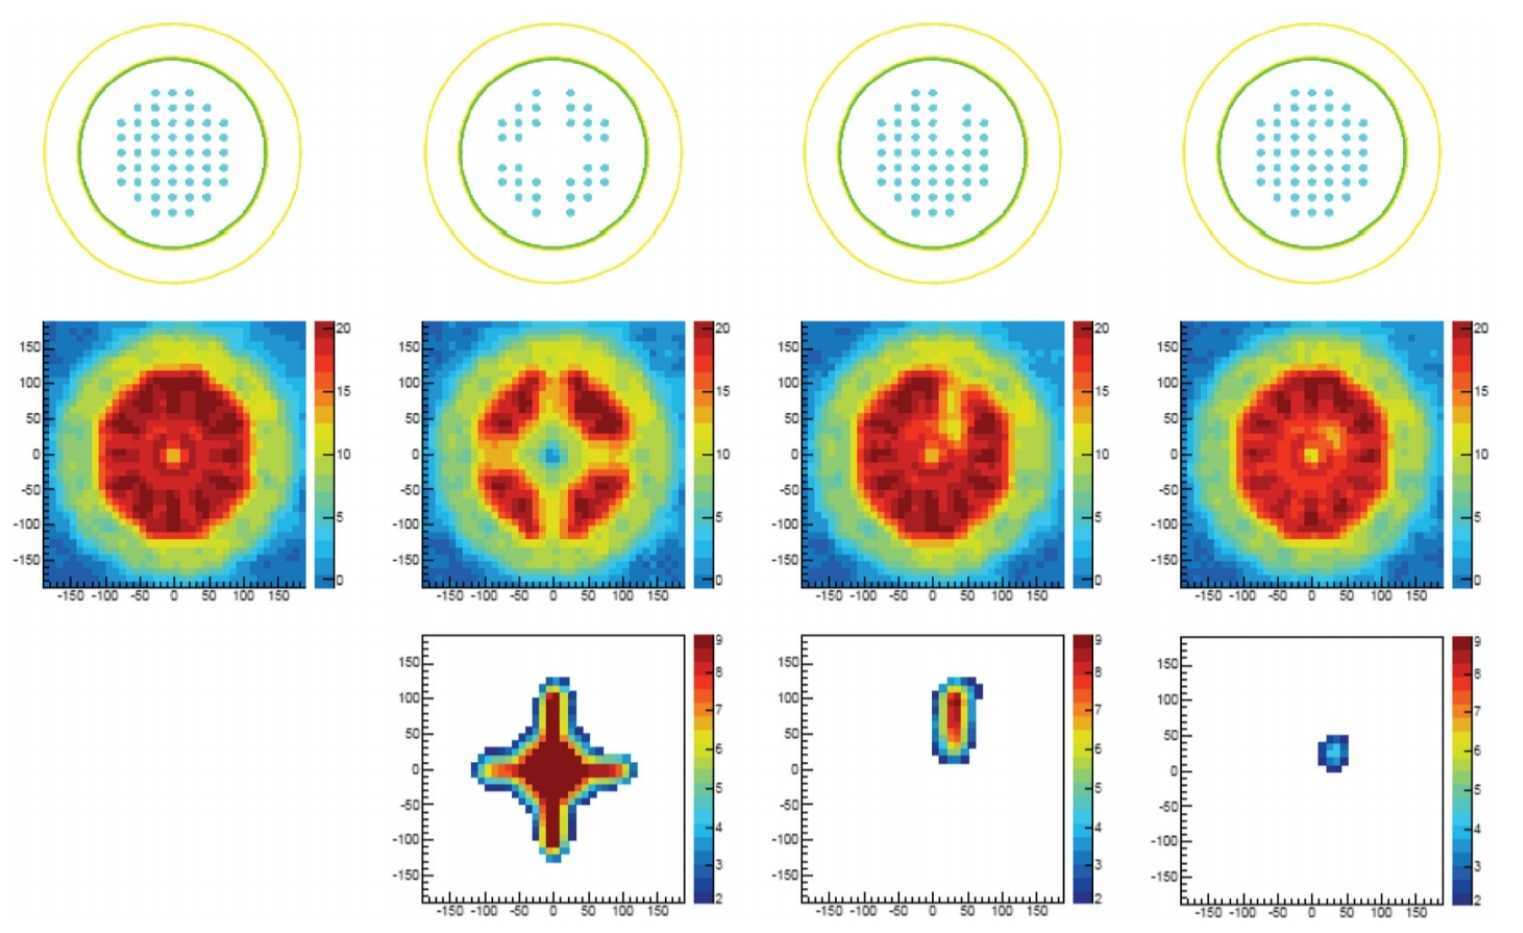
\includegraphics[width=1.0\linewidth]{Chapter5/Figs/MuTomographyExamples/Zed2OstSimulation.jpg}
 \captionof{figure}[Generated GEANT4 distributions for the ZED-2 research reactor.]{Generated GEANT4 distributions for the ZED-2 research reactor. Top row: top-down projection of four different fuel channel configurations. Middle row: reconstructed images using 12 angles of detector and 1 iteration of the ART algorithm. Bottom row: background-subtracted images w in which the leftmost fuel configuration was used as the control case; the missing fuel is clearly visible in case. From \cite{Erlandson_reactorOST_2018}.} 
 \label{fig:Zed2OstSimulation}
\end{figure}

%Imaging a reactor building from differing angles has already been done at the JAPC nuclear
The prospect of imaging dense buildings from differing angles has already been demonstrated by cosmic muon telescopes at the JAPC nuclear power plant (see figure \ref{fig:JapcNuclearPowerImaging} and \ref{fig:3dImagingNFSP}). Even using three positions (see figure \ref{fig:JapcNuclearPowerImaging}) it is possible to combine the detectors to image the nuclear fuel storage pond (NFSP) (see figure \ref{fig:3dImagingNFSP}) \cite{Fujii_ReactorRadiography_2019}. This successful 3D imaging shows a clear use for one-sided reactor muon tomography. The detectors were placed outside the reactor buildings, similar to VIDARR. By using three viewpoints the muon telescopes were able to observe the containment vessel, pressure vessel, and other components of the reactor building \cite{Fujii_ReactorRadiography_2019}. The three views also succeeded in locating two heavy object clusters which were considered to be the nuclear fuel assemblies stored in the NFSP (see figure \ref{fig:3dImagingNFSP}) \cite{Fujii_ReactorRadiography_2019}.

\begin{figure}[!h]
\centering
\begin{minipage}{.45\textwidth}
  \centering
  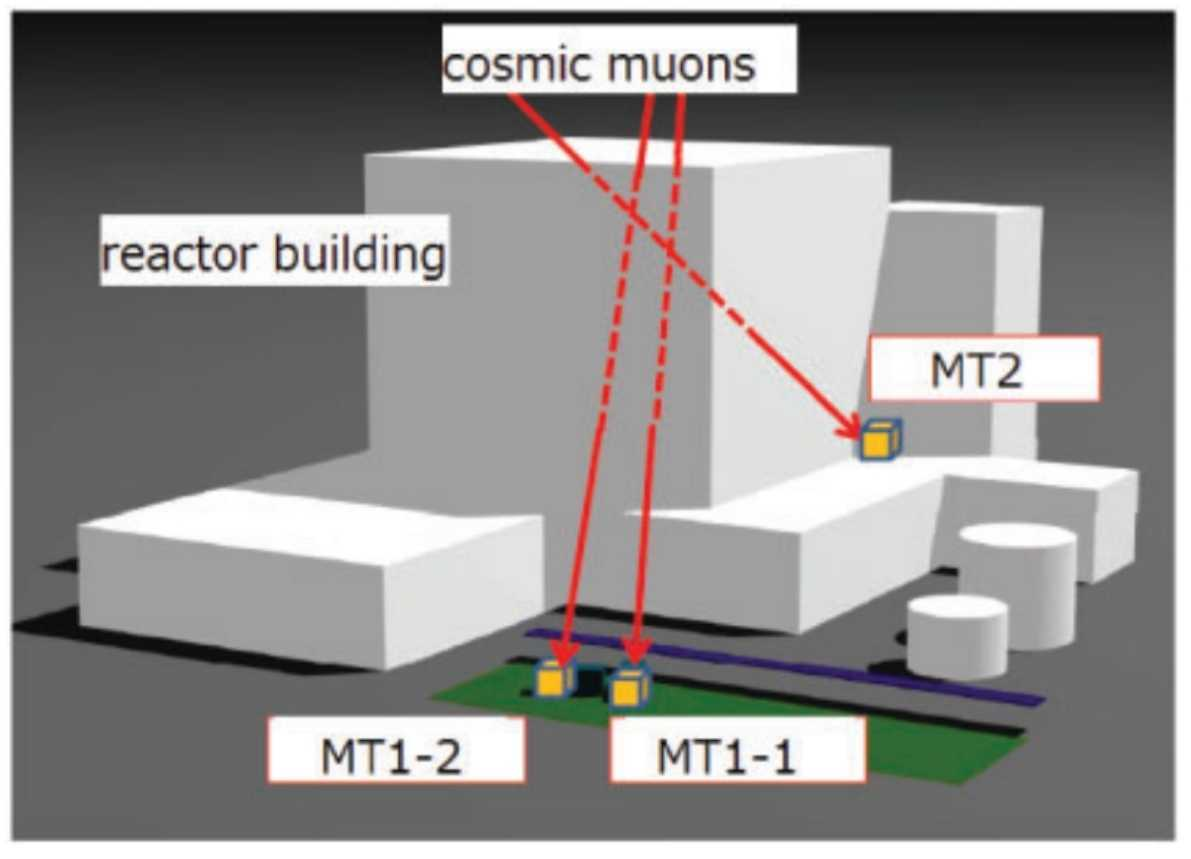
\includegraphics[width=\linewidth]{Chapter5/Figs/MuTomographyExamples/JapcNuclearPowerImaging.jpg}
  \captionof{figure}[Locations of the muon telescopes deployed at the JAPC nuclear power reactor.]{Locations of the muon telescopes (marked as orange cubes) deployed at the JAPC nuclear power reactor. From \cite{Fujii_ReactorRadiography_2019}.} 
  \label{fig:JapcNuclearPowerImaging}
  \vspace{0.956cm} %1 line = 0.478cm % 2 lines = 0.956cm % 3 lines= 1.434cm % 4 lines = 1.912cm % 5 lines = 2.39cm
\end{minipage}%
\qquad
\begin{minipage}{.45\textwidth}
  \centering
  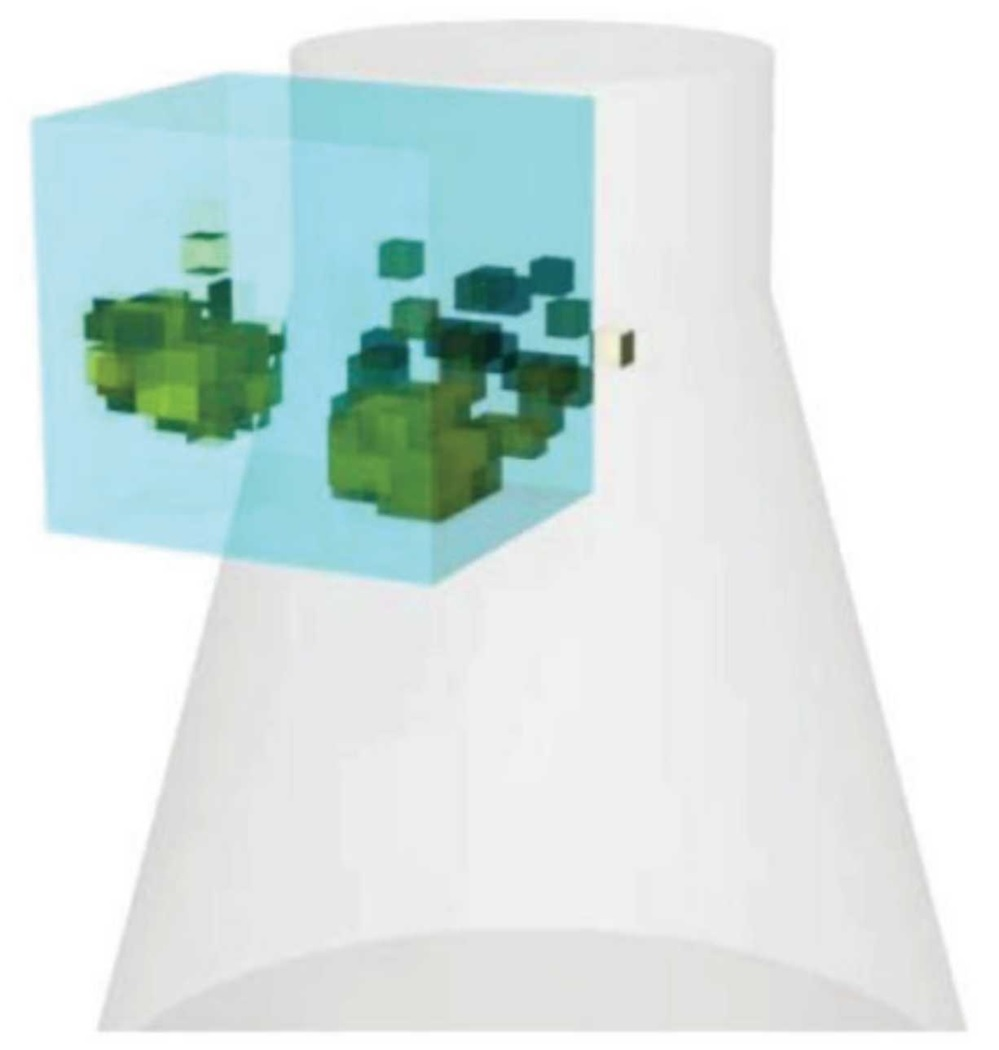
\includegraphics[width=\linewidth]{Chapter5/Figs/MuTomographyExamples/3dImagingNFSP.jpg}
  \captionof{figure}[A 3D image combined image from MT1, MT1-2, and MT2 deployed at JAPC.]{A 3D image combined image from MT1, MT1-2, and MT2 deployed at JAPC nuclear power reactor. The blue area represents NFSP and the green blocks represent areas of high density i.e spent fuel. From \cite{Fujii_ReactorRadiography_2019}.}
  \label{fig:3dImagingNFSP}
\end{minipage}
\end{figure}

%However, clear limitations of this technique are the time required and multiple detectors or deployments. VIDARR can be moved for specific purposes but ideally it should be deployed once and use muon tomography in a brief capacity for positional reconstruction. But this technique would still be possible with VIDARR producing the increased field of view is taken into account. But whether this is desirable will depend on the situations that the VIDARR detector is deployed in the future. 

% \begin{figure}[!h]
%  \centering
%  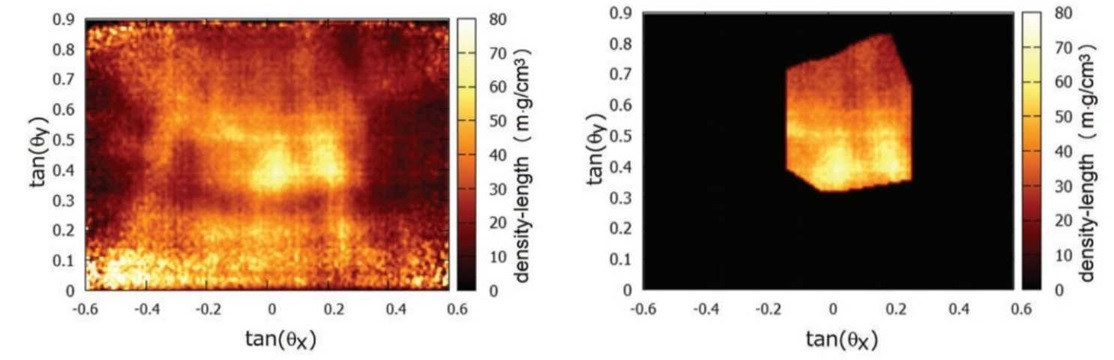
\includegraphics[width=1.0\linewidth]{Chapter5/Figs/MuTomographyExamples/JapcMt2Data.jpg}
%  \captionof{figure}{The density-length distributions estimated from MT2 data: (left) in the entire view area; (right) inside NFSP. From \cite{Fujii_ReactorRadiography_2019}.} 
%  \label{fig:JapcMt2Data}
% \end{figure}

% \begin{figure}[!h]
%  \centering
%  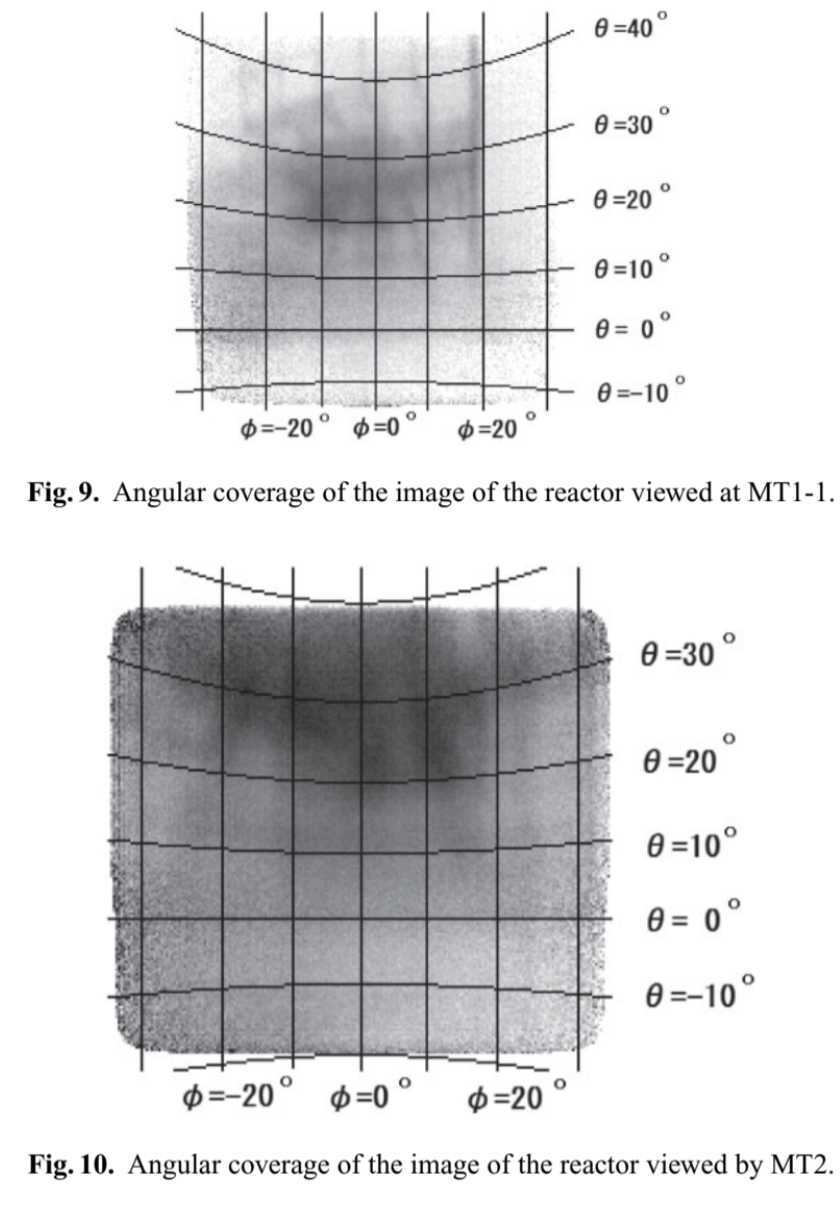
\includegraphics[width=1.0\linewidth]{Chapter5/Figs/MuTomographyExamples/JapcImagingCovering.jpg}
%  \captionof{figure}{.} 
%  \label{fig:JapcImagingCovering}
% \end{figure}

%white space
\vspace{3cm}

% \subsection{Mt. Asama Imaging}
\subsection{Geological One-Sided Muon Tomography}  \label{sec:geologicalTomography} %\label{sec:DIAPHANEmuRadiography}
% One sided 3-d tomography of a volcano fig \ref{fig:mtAsma3dMap}, \cite{Tanaka_mtAsama_2007} 
% \\Muon radiography 
% \\one distant detector fig \ref{fig:MtAsma1dExplanation}
Geological muon tomography relies on imaging large objects, typically volcanoes. In 2007, Mt. Asama in Japan was successfully imaged using an emulsion cloud-chamber sited 1\,km from the (peak of the) mountain. This detector was able to image incoming muon traversing the mountain (see figure \ref{fig:MtAsma1dExplanation}) \cite{Tanaka_mtAsama_2007}. Through the use of muon radiography (determining how much energy the traversing muon particles have lost) an accurate side-on map of rock densities can be produced (see figure \ref{fig:mtAsma3dMap}) \cite{Tanaka_mtAsama_2007}. This side-on tomographic map is highly detailed, requiring the correlation of map data and cosmic muon data. Producing a map with such fidelity is time-consuming, with the time required to resolve a 3\,\% change in density in 1\,km of rock equalling 2 months with a 1000-cm$^2$ detector at solid angle intervals of 0.01 steradians \cite{Tanaka_mtAsama_2007}.

\begin{figure}[!h]
\centering
\begin{minipage}{.45\textwidth}
  \centering
  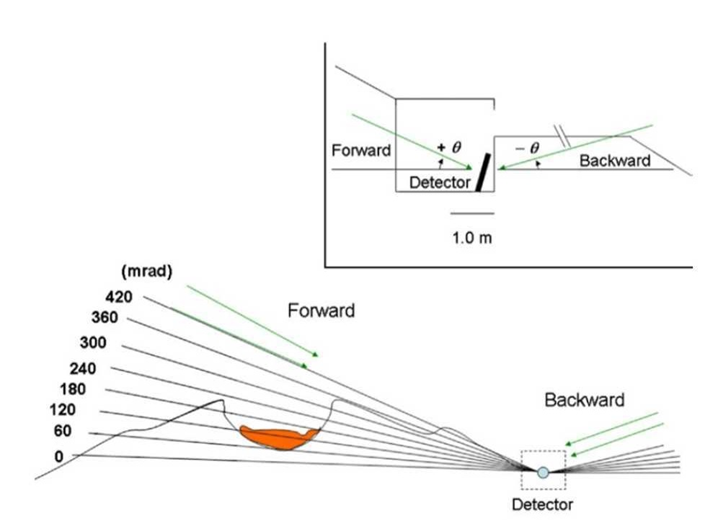
\includegraphics[width=\linewidth]{Chapter5/Figs/MuTomographyExamples/MtAsma1dExplanation.png}
  \captionof{figure}[Cross-section of Mt. Asama showing geometrical arrangements used in the present measurements.]{Cross-section of Mt. Asama showing geometrical arrangements used in the present measurements. The data or muon arriving from the backward direction are also used to confirm the detector efficiency. The inset shows the detector arrangements in the underground space. From \cite{Tanaka_mtAsama_2007}.} 
  \label{fig:MtAsma1dExplanation}
  %\vspace{2.39cm}%5 lines = 2.39cm
\end{minipage}%
\qquad
\begin{minipage}{.45\textwidth}
  \centering
  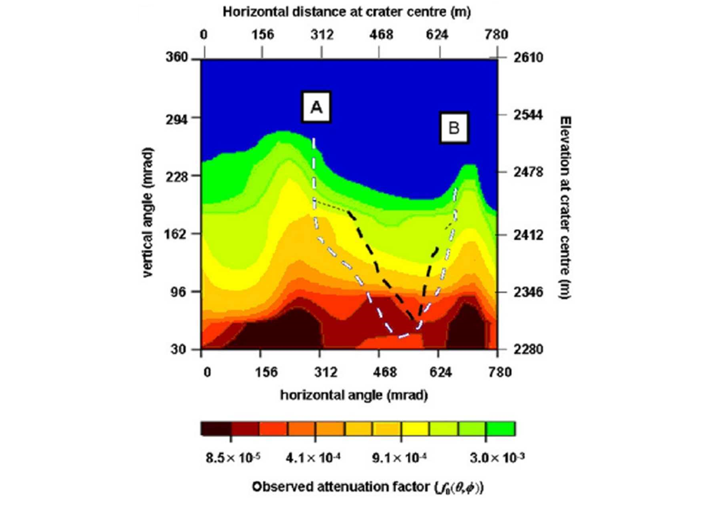
\includegraphics[width=\linewidth]{Chapter5/Figs/MuTomographyExamples/mtAsama1DMuonTomography.png}
  \captionof{figure}[Muon radiographic image of the summit region of Mt. Asama.]{Muon radiographic image of the summit region of Mt. Asama. The position and the shape of the 2003 and 2005 craters are shown by the dashed lines. The points A and B represent the horizontal edge parallel to the Mt. Asama detector. From \cite{Tanaka_mtAsama_2007}.}
  \label{fig:mtAsma3dMap}
  \vspace{0.478cm}
\end{minipage}
\end{figure}

Another prime example of cosmic muon tomography combined with muon radiography is the DIAPHANE collaboration which has a detector that uses plastic scintillating bars and WLS fibres threaded down the centre similar to VIDARR. Instead of using silicon photomultipliers, the DIAPHANE detector uses multianode PMTs to read out the light from the WLS fibres \cite{Marteau_2017}. The DIAPHANE telescope seen in figure \ref{fig:DIAPHANE_deployment} is a series of three planes on a rotating platform with adjustable height. Each plane in DIAPHANE consists of two layers rotated at 90$^\circ$ to each other. The bars in each layer have a rectangular cross section of 5\,cm $\times$ 1\,cm \cite{MARTEAU201223}. 
% Both DIAPHANE and MU-RAY have taken tomographic data to image their surroundings. With DIAPHANE imaging La Soufriere of Guadeloupe using cosmic muon radiography as seen in figure \ref{fig:diaphaneStructualImaging} which shows the different density areas of rock relevant for volcanology \cite{Marteau_2017}.  MU-RAY has also produced similar results for mt. Vesuvius in figure \ref{fig:mtVesuviusMuRayImaging}. Though their technique and data only provide results of rock thickness in meters rather than density \cite{Ambrosino_2014}. Of more interest is figure \ref{fig:mtVesuviusMuRayTransmission} from MU-RAY which shows the ``Transmission'' method. The transmission method used in figure \ref{fig:mtVesuviusMuRayTransmission} is obtained by pointing the MU-RAY detector at the sky for a calibration period of one week then pointing the MU-RAY detector at Mt Vesuvius for one week and then taking the ratio of the two data sets \cite{Ambrosino_2014}. This approach of measuring the free sky and the blocked sky and taking the ratio of the two creates an extremely clear image because it takes the background into account. This creates a clear difference in intensity where transmission of 1 represents the free sky and transmission of 0 represents completely blocked sky. This approach is the one that will be used when analysing the Wylfa reactor site (see chapter \ref{chp:cosmicMuonTomography}) due to the effective reduction of background noise effects and the sharpness of the image it provides. 
% \\\\The DIAPHANE experimental setup seen in figure \ref{fig:DIAPHANE_deployment} shows a cosmic muon telescope with several different planes clearly analysing a very narrow field of view this helps significantly in preventing distortions via bin migration. This is also the case for the MU-RAY collaboration as seen in figure \ref{fig:muRayDetectors} the detector is also multiple flat planes. Each plane in MU-RAY is compromised of triangular prisms with WLS fibres running down the middle (see figure \ref{fig:muRaySetup}). Both MU-RAY and DIAPHANE are traditional cosmic muon telescopes as opposed to VIDARR which is an electron anti-neutrino detector first and a cosmic muon camera second. Despite this DIAPHANE, MU-RAY, and VIDARR all use similar technology: plastic scintillating bars and WLS fibres \cite{Carroll_2018} \cite{Marteau_2017} \cite{ANASTASIO2013423}. DIAPHANE uses ``multianode PMT’s'' to read out information from the WLS fibres \cite{Marteau_2017} whereas VIDARR and MU-RAY use SiPms \cite{Carroll_2018} \cite{ANASTASIO2013423} to read out the information from the WLS fibres. 

\begin{figure}[!h]
 \centering
 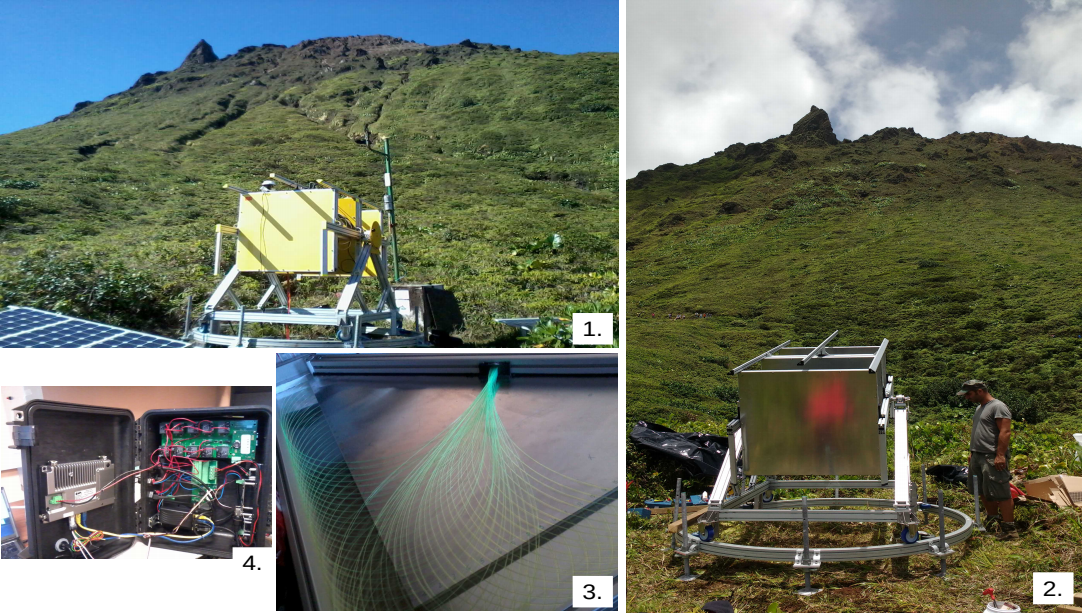
\includegraphics[width=1.0\linewidth]{Chapter5/Figs/Raster/DIAPHANE_deployment.png}
 \captionof{figure}[The deployment of the DIAPHANE detector at La Soufrière of Guadeloupe.]{The deployment of the DIAPHANE detector from \cite{Marteau_2017}. DIAPHANE muon detectors upgrades. 1: the first generation 3 planes muon detector on the slope of La Soufrière of Guadeloupe (PK site). 2: the second-generation 3 planes muon detector, with a transverse segmentation divided by a factor 2, on the slope of La Soufrière of Guadeloupe (SAM site). 3: inner WLS fibres collected on a PMT cookie. 4: compact CTRL BOX with embedded hardened processing unit and electronics: common clock signal, WebRelay, Ethernet switch, Power-over-Ethernet to the wifi antenna. From \cite{Marteau_2017}.} 
 \label{fig:DIAPHANE_deployment}
\end{figure}

%The DIAPHANE detectors are used to image the slope of La Soufrière of Guadeloupe. A volcano of interest. 
The DIAPHANE detectors were used to image the slope of La Soufrière of Guadeloupe, an active volcano through use of cosmic muon radiography. The goal of DIAPHANE is to image the interior structure of the volcano by determining the density of the rock at Guadeloupe. This technique requires a significant amount of time to obtain sufficient clarity. DIAPHANE was deployed between 2010 -- 2016 in which the experiment was able to produce the results seen in figure \ref{fig:diaphaneStructualImaging}. Whilst these results are impressive and give a highly detailed reconstruction, the time frame to achieve these results is very long. 
%For VIDARR this technique would would not be suitable as a time scale for cosmic muon tomography on will be $\sim$ 1 hour per week. However, due to the similar size and shape of the segments between DIAPHANE and VIDARR it's reasonable to conclude that the segmentation effects can be worked around to produce clear images. 

\begin{figure}[!h]
 \centering
 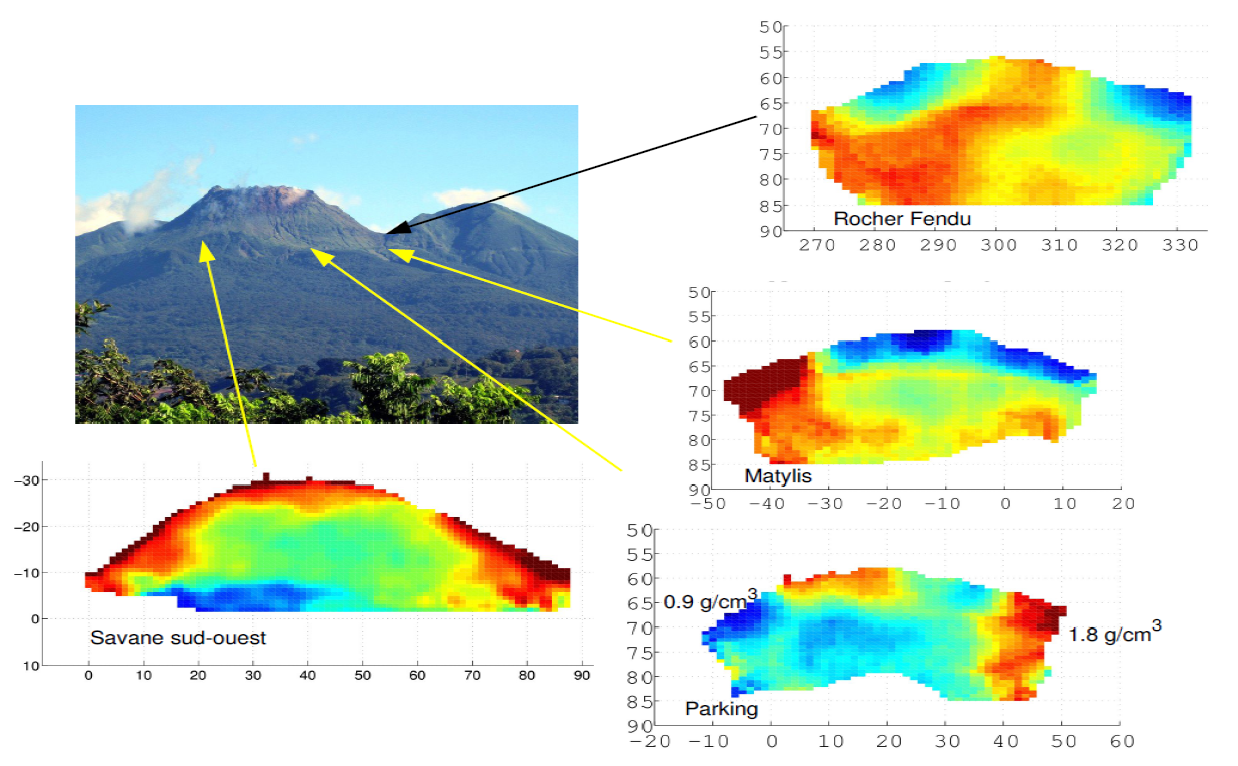
\includegraphics[width=1.0\linewidth]{Chapter5/Figs/Raster/diaphane_structuralImaging.png}
 \captionof{figure}[DIAPHANE structural imaging of the La Soufrière of Guadeloupe dome.]{DIAPHANE structural imaging of the La Soufrière of Guadeloupe dome from 4 different acquisition sites around the dome. The blue areas are the less dense zones of the volcano. The red areas have the highest density. The average density extracted from all those images ranges from 1.6 to 1.8 g.cm$^{-3}$. From \cite{Marteau_2017}} 
 \label{fig:diaphaneStructualImaging}
\end{figure}

% \subsection{MU-RAY Tomography and Transmission Method} \label{sec:murayTomographyAndTransmissionMethod}
%The MU-RAY collaboration also uses cosmic muon radiography to analyse Mt.Vesuvius. 
The results from DIAPHANE are interesting when comparing them from the results from MU-RAY. The MU-RAY detector uses plastic scintillator and silicon photon multipliers (SiPMs) similar to that of VIDARR \cite{ANASTASIO2013423} \cite{Ambrosino_2014}. Apart from the scintillator shape which is the shape of a triangular prism in MU-RAY and the shape of a cuboid in VIDARR, the two use very similar technology. The experimental setup is very similar to that of DIAPHANE with panels arranged with a regular spacing (see Figure \ref{fig:muRayDetectors}). The goals of DIAPHANE and MU-RAY are the same -- to image the interior of volcanoes. MU-RAY even has low power requirements hence solar panels can be used to operate in remote locations \cite{ANASTASIO2013423}. 

% \begin{figure}[!h]
%  \centering
%  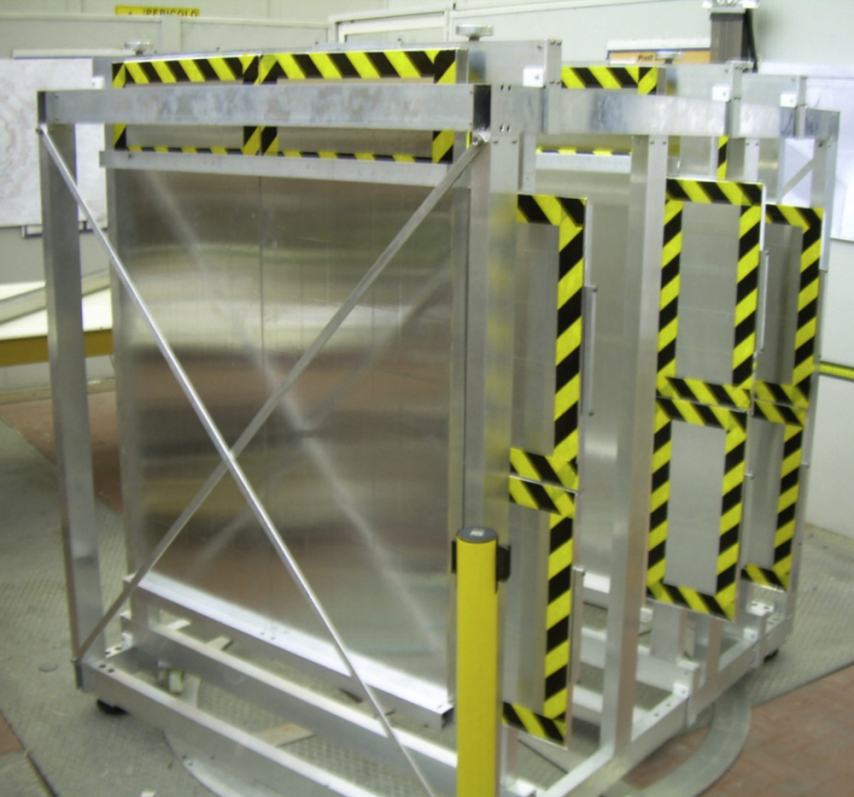
\includegraphics[width=0.5\linewidth]{Chapter5/Figs/Raster/muRayDetectors.png}
%  \captionof{figure}{The MU-RAY detector frame with the three X–Y planes mounted. The frame can be oriented using the rotating platform visible at the bottom. From \cite{ANASTASIO2013423}} 
%  \label{fig:muRayDetectors}
% \end{figure}

The limits of muon radiography are clearly demonstrated by figure \ref{fig:mtVesuviusMuRayImaging}. Whilst the MU-RAY detector was deployed for about 1 month with no obstructions and at an elevation of 800\,m reducing atmospheric scattering, the outline of Mt. Vesuvius is still faint. An increase in rock thickness is clearly visible but no clearly defined features can be seen in figure \ref{fig:mtVesuviusMuRayImaging}. These results are in stark contrast to the DIAPHANE results at Guadeloupe (figure \ref{fig:diaphaneStructualImaging}) which clearly show the interior structure of the volcano. Whilst the technology of DIAPHANE and MU-RAY is not identical they are very similar. DIAPHANE has better energy reconstruction due to the multianode PMT’s as opposed to the SiPMs used in MU-RAY \cite{Marteau_2017}, \cite{ANASTASIO2013423}. However, the spatial reconstruction is superior in MU-RAY as the segments in DIAPHANE have a cross-section of $5\,\textrm{cm} \times 1\,\textrm{cm}$ (5\,cm$^2$) \cite{MARTEAU201223}, whereas the MU-RAY triangular cross-section has a base width of 3.3\,cm and height 1.7\,cm (2.805\,cm$^2$). The lower imaging resolution seen may be ascribed to the combination of worse energy resolution and shorter data collection period. %As a result the blurry resolution in figure \ref{fig:mtVesuviusMuRayImaging} is surprising and leads to the conclusion that the 5 year deployment time for DIAPHANE is the main reason for the sharper resolution in figure \ref{fig:diaphaneStructualImaging}. Positioning is different for each but in both cases the angular size of the Volcano is comparable. 

\begin{figure}[!h]
\centering
\begin{minipage}{.45\textwidth}
  \centering
  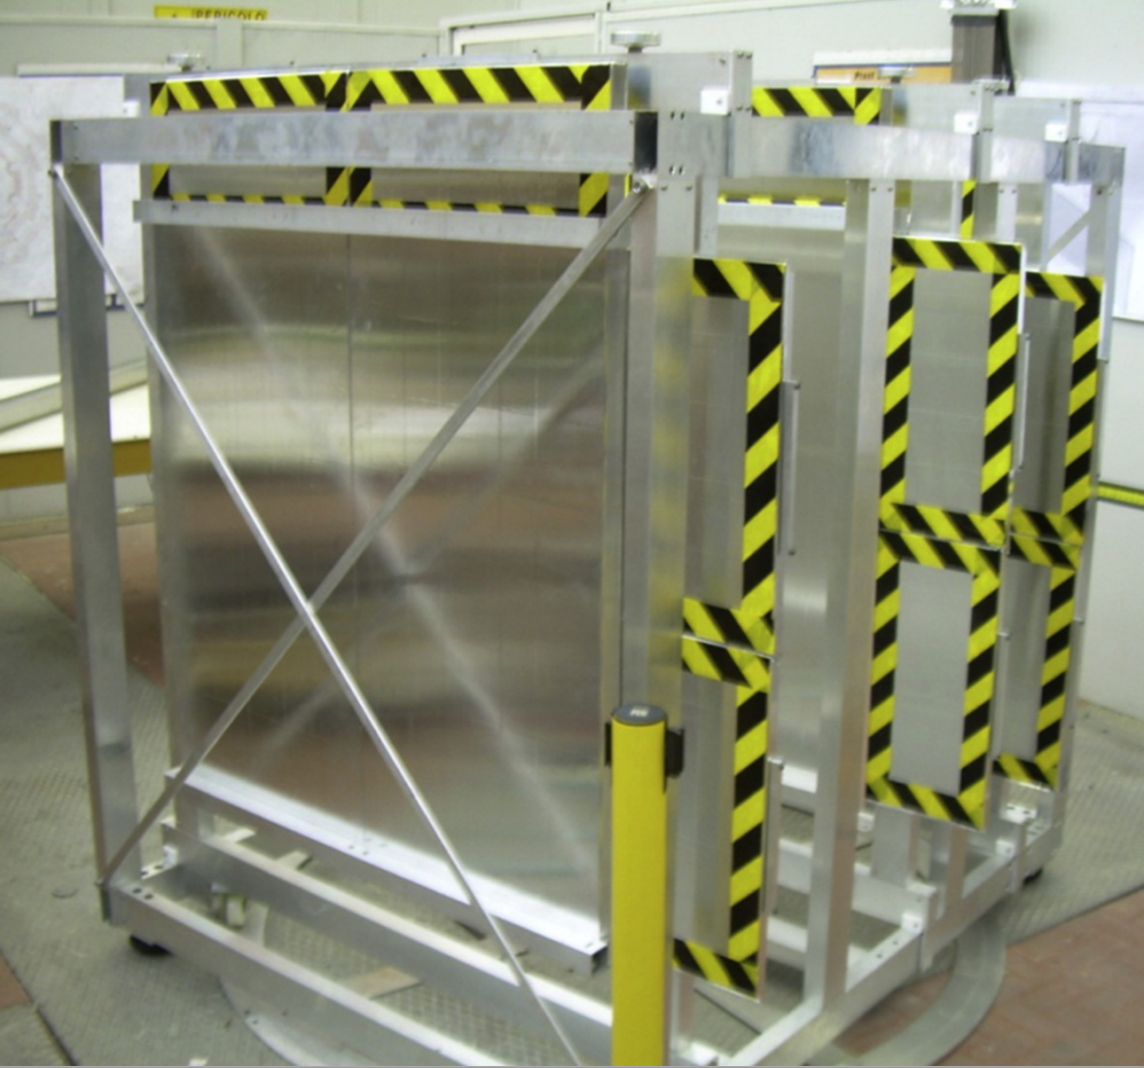
\includegraphics[width=\linewidth]{Chapter6/Figs/Raster/muRayDetectorsAdj.png}
  \captionof{figure}[The MU-RAY detector frame with the three X–Y planes mounted.]{The MU-RAY detector frame with the three X–Y planes mounted. The frame can be oriented using the rotating platform visible at the bottom. From \cite{ANASTASIO2013423}.} 
  \label{fig:muRayDetectors}
  \vspace{0.478cm} %1 line = 0.478cm % 2 lines = 0.956cm % 3 lines= 1.434cm % 4 lines = 1.912cm % 5 lines = 2.39cm
\end{minipage}%
\qquad
\begin{minipage}{.45\textwidth}
  \centering
  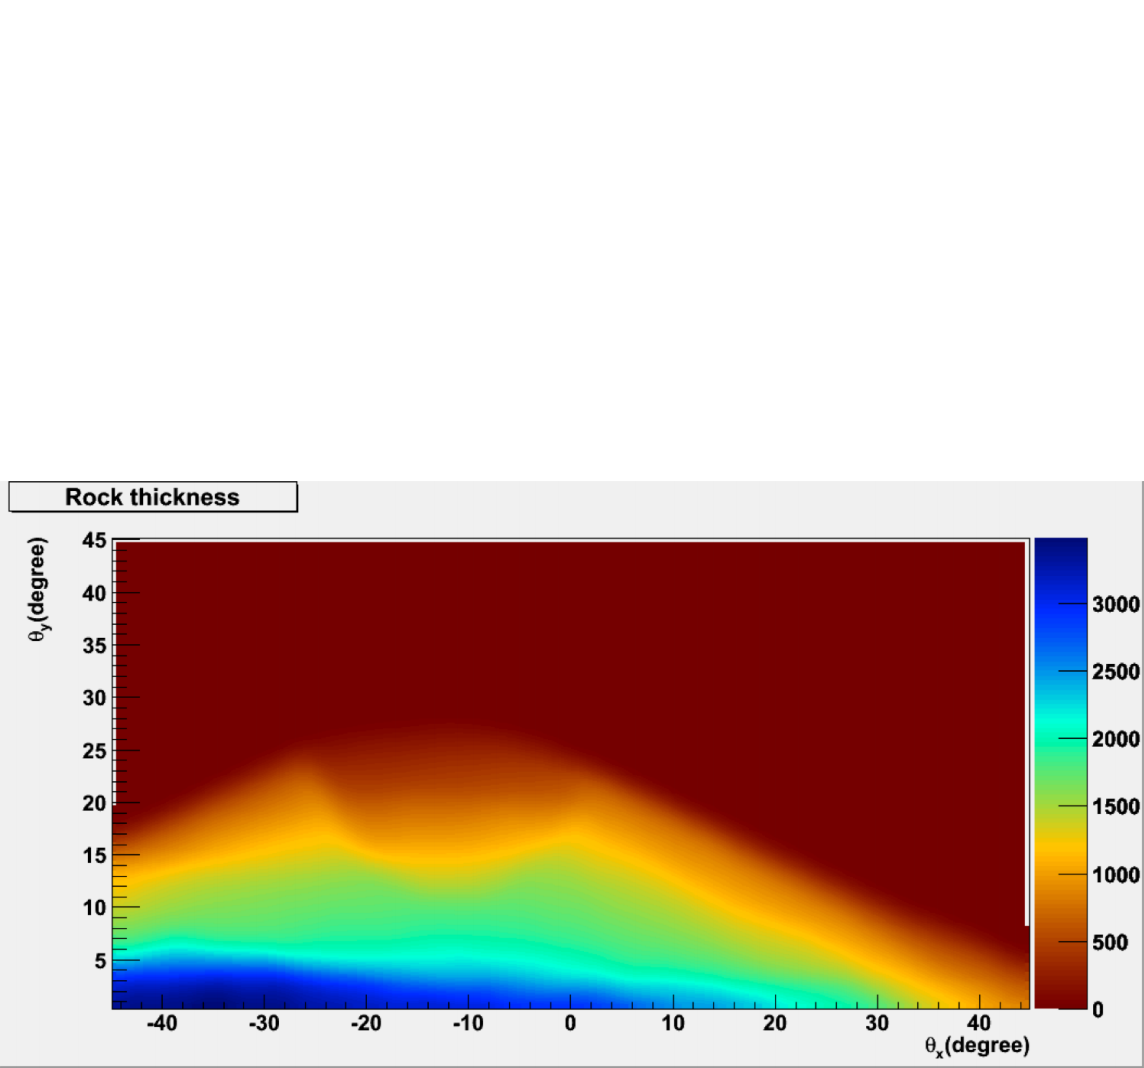
\includegraphics[width=\linewidth]{Chapter6/Figs/Raster/mtVesuviusMuRayImagingAdj.png}
  \captionof{figure}[MU-RAY telescope analysing Vesuvius rock thickness, expressed in m.]{MU-RAY telescope analysing Vesuvius rock thickness, expressed in m, as seen from the observation point at $\sim$ 800\,m altitude. With data taken over a month period of $\sim$ 1 month. From \cite{Ambrosino_2014}.}
  \label{fig:mtVesuviusMuRayImaging}
\end{minipage}
\end{figure}

%As a result of their limited deployment time the MU-RAY collaboration took $\sim$ 1 week to image Mt.Vesuvius using a different technique. The transmission technique. The results of the transmission technique are shown in figure \ref{fig:mtVesuviusMuRayTransmission} whilst this data set has $\sim$ 4 times less live time data than figure \ref{fig:mtVesuviusMuRayImaging} the results are much clearer. The transmission method takes the ratio of the unblocked vertical sky with the area where Mt.Vesuvius is located \cite{Ambrosino_2014}. 
As a result of their limited deployment time the MU-RAY collaboration took about 1 week to image Mt. Vesuvius using a transmission technique. The relative amount of material the muon passed through was found by measuring the proportion of muon stopped in the rock. This was estimated by taking the ratio of the unblocked vertical sky with the area where Mt. Vesuvius is located . This normalisation has the advantage of cancelling acceptance and efficiency dependencies of the detector. But this technique requires the two distributions to be normalised to each other. As a result, the free sky zone common to both histograms should be close to 1 which is shown to be the case in figure \ref{fig:mtVesuviusMuRayTransmission} \cite{Ambrosino_2014}. This is especially useful for cosmic muon tomography with VIDARR as the field of view (FOV) is much wider. Therefore, this technique was utilised when analysing the Wylfa data set.

% \begin{figure}[!h]
%  \centering
%  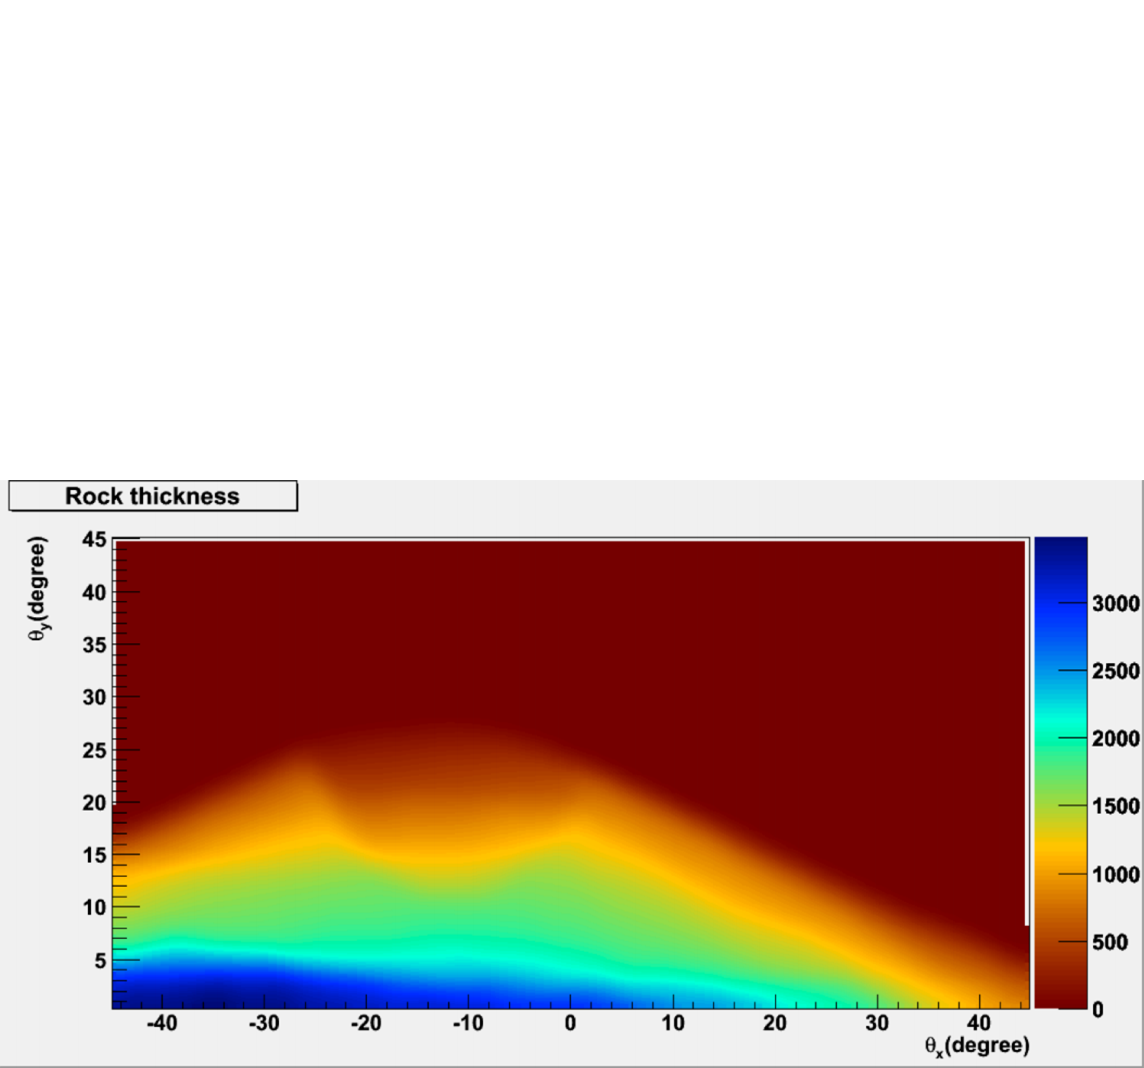
\includegraphics[width=0.6\linewidth]{Chapter5/Figs/Raster/mtVesuviusMuRayImaging.png}
%  \captionof{figure}{MU-RAY telescope analysing Vesuvius rock thickness, expressed in m, as seen from the observation point at $\sim$ 800\,m altitude. With data taken over a month period of $\sim$ 1 month. From \cite{Ambrosino_2014}.} 
%  \label{fig:mtVesuviusMuRayImaging}
% \end{figure}

\begin{figure}[!h]
 \centering
 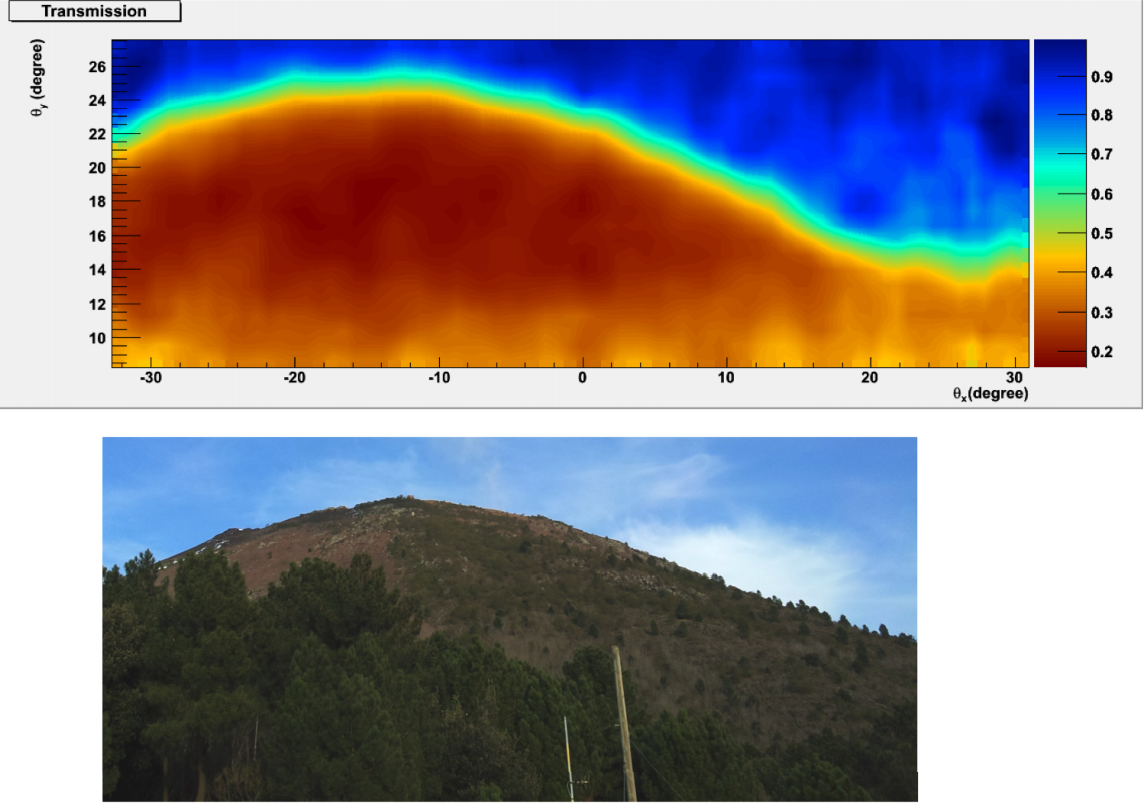
\includegraphics[width=0.8\linewidth]{Chapter5/Figs/Raster/mtVesuviusMuRayTransmission.png}
 \captionof{figure}[MU-RAY data from Vesuvius, transmission histogram compared to a photograph. ]{MU-RAY data from Vesuvius. Top: the transmission histogram of Mt Vesuvius after one week of data taking. Bottom: a picture of Mt Vesuvius taken by the telescope observation point. Taken over a period of $\sim$ 1 week. From  \cite{Ambrosino_2014}.} 
 \label{fig:mtVesuviusMuRayTransmission}
\end{figure}
